\documentclass[12pt,a4paper,twoside,headings=openright]{scrreprt}
% switch to scrbook if you want roman page numbers for the front matter
% however scrbook has no 'abstract' environment!

% binding correction (BCOR) von 1cm für Leimbindung
\KOMAoptions{BCOR=1cm}
\KOMAoptions{draft=no}

\usepackage[utf8]{inputenc} % encoding of sources
\usepackage[T1]{fontenc}
\usepackage{mathtools}
\usepackage{studarbeit}
\usepackage{stmaryrd}
\usepackage{xspace}

\title{Call Arity vs.\\Demand Analysis}
\author{Sebastian~Graf}
\thesistype{Masterarbeit}
\zweitgutachter{Prof.~Dr.~rer.~nat.~Bernhard~Beckert}
\betreuer{Dipl.-Inform.~Denis~Lohner}
\coverimage{fig/combined.png}

% https://tex.stackexchange.com/a/268475/52414
\newlength\stextwidth
\newcommand\makesamewidth[3][c]{%
  \settowidth{\stextwidth}{#2}%
  \makebox[\stextwidth][#1]{#3}%
}
\newlength\smathtextwidth
\newcommand\mathmakesamewidth[3][c]{%
  \settowidth{\smathtextwidth}{$#2$}%
  \mathmakebox[\smathtextwidth][#1]{#3}%
}
\newcommand\mathwithin[2]{%
  \mathmakesamewidth[c]{#1}{#2}
}

% Map Notation
\newcommand{\pfun}{\rightharpoonup}
\newcommand{\emptymap}{[]}
\newcommand{\id}[1]{#1}
\newcommand{\maplit}[3][\id]{\left[#1{#2\mapsto#3}\right]}
\newcommand{\restrict}[2]{#1\restriction_{#2}}

% Semantic sets
\newcommand{\sVar}{\text{\textsf{Var}}}
\newcommand{\sExp}{\text{\textsf{Exp}}}
\newcommand{\sVal}{\text{\textsf{Val}}}
\newcommand{\sGraph}{\text{\textsf{Graph}}}
\newcommand{\sUse}{\text{\textsf{Use}}}
\newcommand{\sUsage}{\text{\textsf{Usage}}}
\newcommand{\sMulti}{\text{\textsf{Multi}}}
\newcommand{\sSig}{\text{\textsf{Sig}}}
\newcommand{\sUseEnv}{\text{\textsf{UseEnv}}}
\newcommand{\sUType}{\text{\textsf{UType}}}
\newcommand{\sUTrans}{\text{\textsf{UTrans}}}
\newcommand{\sTransEnv}{\text{\textsf{TransEnv}}}

% Lattice
\newcommand{\llub}{\sqcup}
\newcommand{\lbiglub}{\bigsqcup}
\newcommand{\lleq}{\sqsubseteq}
\newcommand{\lless}{\sqsubset}
\newcommand{\lTriple}[3]{\left\langle{}#1,#2,#3\right\rangle{}}
\newcommand{\both}{\,\&\,}

% Syntax
\newcommand{\keyword}[1]{\text{\textsf{\textbf{#1}}}}
\newcommand{\sMkPair}{\text{\textsf{(,)}}}
\newcommand{\sApp}[2]{#1\,#2}
\newcommand{\sLam}[2]{\lambda{}#1.\,#2}
\newcommand{\sLet}[2]{\keyword{let}~#1~\keyword{in}~#2}
\newcommand{\sLetRec}[2]{\keyword{letrec}~#1~\keyword{in}~#2}
\newcommand{\sPair}[2]{(#1,#2)}
\newcommand{\sCase}[4]{\keyword{case}~#1~\keyword{of}~\sPair{#2}{#3}\rightarrow#4}
\newcommand{\sITE}[3]{\keyword{if}~#1~\keyword{then}~{#2}~\keyword{else}~{#3}}

\newcommand{\bind}{x_1=e_1}
\newcommand{\binds}{\overline{x_i=e_i}}

% Co-call Graphs
\newcommand{\edge}[2]{#1\text{---}#2}
\newcommand{\neighbors}[2]{N_{#1} ({#2})}
% I'm not happy with the results of this
%\newcommand{\singletonloop}[1]{\mathwithin{#1}{\tikz[baseline={([yshift=-.5ex]current bounding box.center)},every loop/.style={looseness=0.1}]{\node {$#1$} edge [loop above] ()}}}

% Auxiliary Operators
\newcommand{\uscore}[1][\mathunderscore]{\mathwithin{#1}{\mathunderscore}}
\newcommand{\sfop}[1]{\mathsf{#1}}
\newcommand{\dom}[1]{\sfop{dom}\,#1}
\newcommand{\zap}{\sfop{zap}}
\newcommand{\expand}{\sfop{expand}}
\newcommand{\letup}[2]{#1\!\uparrow_{#2}}
\newcommand{\letdown}[2]{#1\!\downarrow_{#2}}
\newcommand{\liftstar}[1]{[#1]^*}
\newcommand{\liftqm}[1]{[#1]^\sfop{?}}
\newcommand{\cmblet}[2]{#1\ltimes#2}
\DeclareMathOperator{\lfp}{lfp}
\newcommand*{\cf}{cf.\@\xspace}
\newcommand*{\vs}{vs.\@\xspace}
\newcommand*{\eg}{e.g.\@\xspace}
\newcommand*{\ie}{i.e.\@\xspace}

% Transfer function
\newcommand{\transfer}[2]{\mathcal{T}\llbracket#1\rrbracket_{#2}}
\newcommand*{\letupsc}{\textsc{LetUp}\xspace}
\newcommand*{\letdnsc}{\textsc{LetDn}\xspace}
\newcommand{\fix}{\keyword{fix}\xspace}
\newcommand{\up}{\sfop{up}}
\newcommand{\down}{\sfop{down}}


\begin{document}

\begin{otherlanguage}{ngerman} % Titelseite ist immer auf Deutsch
\mytitlepage
\end{otherlanguage}

\begin{abstract}
\begin{center}\Huge\textbf{\textsf{Zusammenfassung}}
\end{center}
\vfill

  Optimierungen in Compilern für funktionale Programmiersprachen verlassen sich auf gute Schätzungen dafür, wie oft syntaktische Konstrukte relativ zum umgebenden Kontext ausgewertet werden.
  Eine \emph{Kardinalitätsanalyse} berechnet untere und obere Schranken für diese Auswertungsmultiplizitäten.
  Während untere Schranken genau den Ergebnissen einer \emph{Strictness Analyse} entsprechen, berechnen \emph{Usage Analysen} obere Grenzen.

  Der Glasgow Haskell Compiler (GHC) integriert zwei Analysen, Call Arity und Demand Analysis, die beide unabhängig voneinander Usage Resultate berechnen.

  Diese Arbeit stellt eine Usage Analyse vor, die ihr Gegenstück in beiden Analysen verallgemeinert.
  Eine komplexe Analysereihenfolge hat zu einem neuartigen, graphbasierten Ansatz zur Fixpunktiteration geführt, losgelöst vom Syntaxbaum.
  Saubere Trennung von Analyselogik und Aufbau des Datenflussnetzwerks wird durch eine eingebettete domänenspezifische Sprache gewährleistet.
  
\vfill

  Optimisation passes in compilers for functional languages rely on good estimates for how often some syntactic construct is evaluated relative to its enclosing context.
  A \emph{cardinality analysis} computes lower and upper bounds to these relative evaluation multiplicities.
  While the lower bounds correspond to the results of a \emph{strictness analysis}, the upper bounds are computed by \emph{usage analyses}.

  The Glasgow Haskell Compiler (GHC) integrates two analyses, Call Arity and Demand Analysis, that compute usage results independently of another.

  This thesis introduces a usage analysis that generalises its counterpart in both analyses.
  Challenges in analysis order necessitated a novel graph-based approach to fixed-point iteration, detached from the syntax tree.
  An embedded domain specific language cleanly separates construction of the data-flow framework from analysis logic.

\vfill

\end{abstract}

\tableofcontents

\chapter{Introduction}\label{sec:intro}

High-level programming languages abstract from operational details so that the programmer can focus on solving problems instead of fighting with the concrete hardware the solution is supposed to run on.

Haskell, being a non-strict functional programming language, is an extreme example of this, going well beyond common features such as garbage collection.
Rather than encoding a program as an imperative sequence of commands to execute, programs are specified declaratively as a pure expression to evaluate.

Non-strictness demands that evaluation is driven entirely by the need to make progress in evaluating this top-level expression.
The call-by-need evaluation strategy employed by implementing compilers such as the Glasgow Haskell Compiler (GHC) guarantees that no expression is (observably) evaluated that is not needed over the course of executing the program!

This most immediately affects programmers in freeing them from thinking long and hard whether some definition should be floated nearer to its use site, to avoid unnecessary evaluation.
But laziness also provides huge benefits when it comes to composibility:
In Haskell, \hsinl{take k . sort} exhibits the same asymptotics as a Top-N query implemented directly\footnote{With a selection algorithm based on the sorting algorithm used to implement \hsinl{sort}, that is.}. 
Strict programming languages usually provide additional functions for handling these important cases, expecting the library designer to anticipate different user scenarios.
In short, laziness allows to compose small bits of functionality into bigger programs, without paying in asymptotic complexity.

Some purely functional data structures even benefit from laziness in a logarithmic factor, bringing persistent data structures on par with their mutable counterparts.
As \textcite{pippenger} and \textcite{bird} show, this is not always possible in a purely functional setting without laziness.

As with most high-level abstractions, lazy evaluation is not free, however.


\chapter{Preliminaries}\label{sec:prel}

This chapter will start out by laying out some ground work for later sections.

There seems to be no ubiquitous domain language on the various cardinality analyses floating around in papers over the years \parencite{projimpl,verstoepthesis,sestoft,sharing,updabs,callarity,warnsbrough,dmd,card}, so \cref{sec:zoo} will provide a glossary for that.

We'll give abridgements of the two analyses we aim to generalise in \cref{sec:callarity} and \cref{sec:dmd}.

\section{Analysis Zoo}\label{sec:zoo}

Prior work disagrees in what meaning they assign to different concepts related to analyses that track evaluation counts in some way.

Just to name an example, the concept of \emph{demand} within GHC refers to a pair of strictness and usage information, while \textcite[Appendix~C.2]{warnsbrough} defined demand as evaluating a binding to weak head normal form (WHNF), as opposed to applying the bound expression to one argument (\emph{use}).

\subsection{Cardinality Analysis}\label{sec:card}

A \emph{cardinality analysis} answers questions regarding how often some syntactic thing is used with respect to a single evalutation of the outer context.

Let us understand this by examining the following example:

\begin{haskellcode}
  main = do
    let a = ...
        b = ...
        c = ...
        d = ...
        e = ...
    print (a + if b then a*d else c*c)
\end{haskellcode}

A sophisticated compiler for a lazy language can find out the following facts, always assuming a single execution of \hsinl{main}:
\begin{itemize}
  \item The binding for \hsinl{a} is evaluated at least once.
  \item The binding for \hsinl{b} is evaluated exactly once.
  \item The binding for \hsinl{c} is either evaluated twice or not at all.
  \item The binding for \hsinl{d} is either evaluated once or not at all.
  \item The binding for \hsinl{e} is absent, \eg not used even once.
\end{itemize}

Based on these facts, the compiler can apply a number of optimisations:
\begin{description}
  \item[Call-by-value] 
    Since \hsinl{a} and \hsinl{b} are evaluated \emph{at least once}, the compiler is free to apply a call-by-value evaluation strategy for them.
    Recovering strictness in this way makes a huge difference, as subsequent transformations such as a worker/wrapper transformation \parencite{ww} may exploit this information to great effect.
  \item[Call-by-name]
    Because \hsinl{b} and \hsinl{d} are evaluated \emph{at most once}, the compiler can employ a call-by-name strategy instead of call-by-need.
    Operationally, this omits unnecessary thunk updates for these so-called \emph{single-entry} thunks, because the computed value doesn't need to be memoised.
  \item[Absence]
    The example doesn't mention any use of \hsinl{e}. 
    Such absence can be exploited by not generating code for the binding at all, or replace the binding by an error message in case of analysis failure.
    Absence is also important for the worker/wrapper transformation \parencite{ww}, in that it conjures custom calling conventions that won't need to mention (partially) absent arguments at all.
\end{description}

Of course, call-by-value and call-by-name are mutually exclusive, which means that for \hsinl{b} the compiler must choose between the two. 
In practice, that is an easy choice: 
Call-by-value enables much more effective optimisations than call-by-name.
Nonetheless, the share of single-entry thunks is dominating (70\% according to same dated results of \textcite{updabs}) and deemed worth optimising.

Note that we only care for the three cardinalities $\{0, 1, \omega\}$ in our examples:
Everything beyond the second evaluation carries no usable information, thus we denote the cases of `evaluated multiple times' with $\omega$.

As in the above example, possible cardinality may also depend on runtime information, so that information is better reflected as a subset of $\{0, 1, \omega\}$.
Most interesting, however, are the over-approximating (\eg maximum) and under-approximating (\eg minimum) cardinalities, which act as proofs for the compiler to justify said optimisations.

Thus, a cardinality analysis assigns each binding an interval of its maximum und minimum evaluation cardinality, relative to a single evaluation of the binding site.

In the example above, \hsinl{a} would be annotated with $[1,\omega]$ (evaluated at least once, possibly many times), whereas the absent \hsinl{e} would be annotated with $[0, 0]$ (evaluated at most never).

This is exactly the notion of usage-interval analysis in \textcite[Chapter~5]{sestoft}, which defines `usage count' as what we call cardinality.

\subsection{Strictness Analysis}\label{sec:strict}

Analogous to the distinction of alias analyses between \MayAlias and \MustAlias in typical imperative languages, cardinality analysis can be split in two separate passes, \MinCard and \MaxCard. 
Looking at the \MinCard problem, the only information that is exploited by compilers so far is that of \emph{strictness}.

An expression \hsinl{... let x = e in body ...} is strict in the binding \hsinl{x} if the whole expression diverges whenever \hsinl{e} does.
Put another way: 
If an expression is \emph{strict} in some binding \hsinl{x}, the expression will certainly evaluate \hsinl{x} on all code paths, \eg \hsinl{x} is evaluated at least once.

Finding out whether or not a binding is evaluated at least once, relative to a single evaluation of the binding expression, is the goal of \emph{strictness analysis}.
Strictness analysis enables the call-by-value optimisations explained above and caters for the worker/wrapper transformation \parencite{ww}, sketched out in \cref{sec:ww}.

Note that from a \MinCard perspective, there is at least one more bit of information that would also be of interest, namely if a binding is evaluated \emph{at least multiple times} (\eg annotation $[\omega,\omega]$).
There is no real gain for compilers in knowing that information!
This leads to delightful simplicity in the implementation of strictness analysis compared to \MinCard or \MaxCard in the case of thunks (\cf \cref{sec:untangle}).

\subsection{Usage Analysis}\label{sec:usage}

Strictness analysis captures all necessary information on \MinCard, \eg if $\alpha$ in the annotation $[\alpha,\beta]$ is $0$ or $1$.

We refer to the analogue of \MaxCard as a \emph{usage analysis}.
A usage analysis provides an over-estimate to cardinality.
For a given binding, it finds out \emph{at most} how often the binding is evaluated in a single evaluation of the binding expression.

Both \emph{absence analysis} (\eg, is $\beta$ in the cardinality annotation $[\alpha, \beta]$ at most 0?) and \emph{sharing analysis} (\eg, is $\beta$ in the cardinality annotation $[\alpha, \beta]$ at most 1?) are generalised by usage analysis.

The results of a sharing analysis support the call-by-name optimisation from above, while absence information is needed together with strictness information for the worker/wrapper transform.

As \textcite[Section~2.4]{verstoep} points out, a sharing analysis finds out similar results as a static analysis based on \emph{uniqueness types}.
They serve different purposes, however; Uniqueness information is propagated during type-checking and may affect which programs are rejected, while sharing analysis is an enabling analysis for other optimisations in the middleend.

That also means that the benefits of uniqueness types might carry over to thunks that a sharing analysis finds to be single-entry, just by changing their type after it passed type-checking.
\textcite{sharing} give an overview over commonalities and differences of sharing analyses and uniqueness types and provide an analysis generalising both.

Less far-fetched is the benefit of identifying \emph{one-shot} lambdas.
Roughly speaking, a lambda is one-shot if a single evaluation of the expression that reduces to the lambda leads to at most one call of the lambda.

This is best understood by an example.

\begin{example}
  Consider the function \hsinl{f} in the following expression:
  \begin{haskellcode}
    let f x y = m*x + y
    in f 1 2 + f 3 4
  \end{haskellcode}

  The outer lambda, binding \hsinl{x}, is not one-shot:
  As the work of evaluating the expression bound to \hsinl{f} to WHNF (which it trivially has) is shared between the two calls to the lambda.

  It is different for the inner lambda, binding \hsinl{y}, however.
  In each of the two calls, the result of applying \hsinl{f} to one argument is immediately applied to another argument. The redexes \hsinl{f 1} and \hsinl{f 2} represent the relative evaluations here and in each case the resulting lambda is called once.
  
  Thus, the lambda which binds \hsinl{y} is one-shot.
\end{example}

Recognising one-shot lambdas opens up opportunities for a number of further optimisations \parencite[Section~6.6.2]{warnsbrough}:
\begin{description}
  \item[Floating]
    Normally, floating a \hsinl{let} binding inside a lambda risks duplicating shared work.
    One-shot lambdas guarantee that the body will not be evaluated more often than the containing expression, so floating bindings inside is safe.

    Note that in the above example, \hsinl{m} could not be floated inside the body of \hsinl{f}.
    Although the inner lambda (\hsinl{y}) is one-shot, the outer isn't.
  \item[$\eta$-expansion]
    Instead of floating \hsinl{let} bindings (and other syntactic things) inside a one-shot lambda, we can go the other way and float inner one-shot lambdas \emph{out}.
    This process is called $\eta$-\emph{expansion}, as opposed to $\eta$-reduction.
    $\eta$-expansion is not generally safe for ordinary lambdas for the same reasons as floating \hsinl{let} bindings in is not, \eg possible duplication of work.

    $\eta$-expansion based on usage information is the key idea behind the efforts of \textcite{callarity} of making \hsinl{foldl} a good consumer for list fusion.
  \item[Inlining]
    Inlining bindings under a lambda risks duplication of shared work, which is why the inliner needs additional confirmation that the chain of lambdas under which to inline is one-shot.
    There is large overlap with the float in case, but remember that inlining may be beneficial in cases where a binding cannot be floated in.
\end{description}

All these opportunities boil down to the compiler being cautious not to duplicate work when shoving something under a lambda.
It seems reasonable to annotate one-shot lambdas while performing usage analysis as the information falls off as a by-product anyway.

\subsection{Arity Analysis}\label{sec:arity}

We close by characterising \emph{arity analyses}, a concept unrelated to cardinality on first sight.

An arity analysis annotates bindings with the number of value arguments they can be applied to before doing any non-negligible work.

The simplest possible arity analysis would just count the leading chain of lambdas in the bound expression to ascribe bindings with this \emph{manifest arity}.
\begin{haskellcode}
  let f b = 
        if b
        then id 
        else (*2)
  in f True 2
\end{haskellcode}

Here, \hsinl{f} has manifest arity 1.
While this starts out as a rather manageable analysis, GHC's arity analysis is much more involved, having to deal with coercions, instrumentation and cost models.

In the above example, GHC would consider the \hsinl{if} expression matching on a variable cheap to duplicate and thus \emph{expand} \hsinl{f}'s \emph{arity} (by $\eta$-expanding its bound expression) to two.

\section{Worker/Wrapper Transformation}\label{sec:ww}

Discussing a transformation in a chapter that is all about analyses seems out of place, but we refer to the worker/wrapper transformation quite often and this seems like the best place to sketch out its idea.
A detailed treatment can be found in \textcite{ww}.

Consider the following function and its usage:
\begin{haskellcode}
  f (a, b) = 
    <large body mentioning b>

  main = print (f (4, 5))
\end{haskellcode}

There is some pointless packing involved in calling \hsinl{f} with the pair literal:
After all, \hsinl{f} immediately unpacks the pair when called!
Also, since \hsinl{a} is not used by \hsinl{f} in the first place, it would be enough to pass \hsinl{b}.

If \hsinl{f} can be inlined, this packing/unpacking immediately gets optimised away by the simplifier.

If \hsinl{f} cannot be inlined (it may be recursive or its body too big), then the compiler has to leave the call site untouched.
That's a shame, since the repeated boxing and unboxing performs needless allocation, which especially hurts in hot loops.

The common solution to this problem is to apply a \emph{worker/wrapper split} to the function:
\begin{haskellcode}
  f (a, b) = 
    $wf b

  $wf b =
    <large body mentioning b>

  main = print (f (4, 5))
\end{haskellcode}

This makes \hsinl{f} only a thin \emph{wrapper} over the actual \emph{worker} function \hsinl{$wf}, which only takes those components of the pair it really uses (\hsinl{b}, that is).
Now, \hsinl{f} is really cheap and will always be inlined at call sites, so the needless boxing and unboxing vanishes.
Effectively, the inlinable wrapper exposes a specialised \emph{calling convention} for the worker function.

This works even in the face of recursion, where the wrapper can be inlined within the body of the worker to reduce allocations.

The worker/wrapper transformation is paramount to performance in a non-strict language like Haskell. 
In order to justify unboxing primitives like machine integers (which can be treated like 1-tuples), a strictness analysis must approve the strictness in the (generally lifted) argument to unbox.
An absence analysis can identify which parts of a record (like \hsinl{a} above) are not used at all by the function, so that the number of arguments passed to the worker is kept minimal.
Without this transformation and its interplay with strictness, GHC could never reach performance within the same magnitude as C.

\section{Call Arity}\label{sec:callarity}

Call Arity \parencite{callarity} is a carefully crafted analysis within GHC, motivated by making \hsinl{foldl} take part in list fusion without compromising in terms of allocations.

It does so by $\eta$-expanding bindings based on usage information.
This is best demonstrated by an example:
\begin{haskellcode}
  let f x = 
        if expensive
        then id 
        else (*2)
  in f 1 2 + f 4 5
\end{haskellcode}

Call Arity recognises \hsinl{f} as always being called with two arguments and justifies $\eta$-expansion of the expression bound to \hsinl{f} to arity two.
The justification for why this doesn't lose shared work of evaluating the arbitrarily \hsinl{expensive} expression (\cf \cref{sec:usage}) is that there is no call with arity less than two, so that the sharing would never be observed.

This would be all there is to arity expansion (\eg $\eta$-expansion of the bound expression) based on usage, if it weren't for thunks:
\begin{haskellcode}
  let f =
        if expensive
        then \x y -> y
        else \x y -> y*2
  in f 1 2 + f 4 5
\end{haskellcode}

This computes the same expression as the previous example, but has different operational behavior.
Since \hsinl{f} is now a thunk (\eg binds an expression that is not in WHNF), expanding \hsinl{f} to \emph{call arity} -- the minimum arity of each call, as opposed to Call Arity, the analysis -- duplicates the work associated with evaluating \hsinl{expensive}. 
This work would otherwise be shared between the two calls and unsharing it may in general degrade performance by an arbirary amount.

It is safe to $\eta$-expand thunks to call arity if they are called just once, though:
\begin{haskellcode}
  let f =
        if expensive
        then \x y -> y
        else \x y -> y*2
  in if b then f 1 2 else f 4 5
\end{haskellcode}

This also demonstrates that \hsinl{f} can't be inlined due to imminent explosion in code size.

Thus, Call Arity tracks in its abstract domain for each binder whether it was called only once and the call arity (as in minimum arity of each call).
The `called once' part is tracked by a sharing analysis, while call arity is computed by a simple arity analysis.

As the examples demonstrate, the arity analysis leans on the sharing analysis.
The next example shows that information also flows in the reverse direction:
\begin{haskellcode}
  let f x = expensive
  in f 1
\end{haskellcode}

A (rather simple) sharing analysis would analyse the binding of \hsinl{f} and would have to assume that \hsinl{expensive} is evaluated possibly multiple times, because it is hidden under a lambda.
Under the assumption that \hsinl{f} is only called once, with one argument (!), the sharing analysis can conclude that \hsinl{expensive} is only used once.

Thus, the interleaving of sharing and arity analysis within Call Arity makes sense, although as we see later in \cref{sec:generalise}, call arity is just the result of exploiting one-shot and single-entry information.\smallskip

In order for Call Arity to have available the minimum call arity of an identifier when analysing its bound expression, it has to analyse \hsinl{let} from the bottom up, \eg analyse the body before the bound expression.

This has limitations in cases like this:
\begin{haskellcode}
  let x = ...
  in let y = 2*x
     in if b
        then x
        else y
\end{haskellcode}

Here, the bottom-up sharing analysis will not find out that \hsinl{x} is only evaluated once. 
At the point where \hsinl{y} is analysed, it is already clear that \hsinl{x} was evaluated, and because \hsinl{y} was also evaluated, it seems that \hsinl{x} was evaluated twice.
That is too conservative, however: The bottom-up scheme forgot that \hsinl{y} and \hsinl{x} were evaluated on different code paths.

Thus, Call Arity employs a novel sharing analysis based on \emph{co-call graphs} instead.
Co-call graphs track which identifiers are possibly evaluated with each other by an edge.
The absence of a co-call edge proves that the unrelated identifiers are never evaluated on the same code path.

For the \hsinl{if} expression in the above example, the co-call graph looks like this:
\[  
  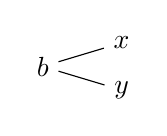
\begin{tikzpicture}[baseline={(0.base)}]
    \node (0) {$b$};
    \node at (1,0.3) (1) {$x$};
    \node at (1,-0.3) (2) {$y$};
    \draw (0) -- (1);
    \draw (0) -- (2);
  \end{tikzpicture}
\]

It properly reflects that \hsinl{x} is never called together with \hsinl{y}.
The analysis then makes use of that information when handling the \hsinl{let} expression binding \hsinl{y}, by effectively performing substitution of the co-call graph of its bound expression (which contains the single node \hsinl{x} without any edges) for \hsinl{y} in the above co-call graph of the body.

After this substitution step, there will be no loop on \hsinl{x}, because there was no edge between \hsinl{y} and \hsinl{x}.
This represents the fact that \hsinl{x} is not called with itself, or only called once, plainly speaking.

Co-call graphs and this rather involved substitution procedure are illuminated in detail in \cref{sec:graph} and \cref{sec:let}.
\Cref{sec:bench} discusses the impact of co-call graphs on analysis precision and performance.

\section{Demand Analyser}\label{sec:dmd}

GHC's approach to strictness and usage analysis is that of \emph{demand analysis}.

It is what we referred to as a cardinality analysis (\cref{sec:card}), integrating both \MinCard and \MaxCard analyses.
To make matters more confusing, the part concerning usage analysis is introduced in \textcite{card}, titled `Modular, Higher-order Cardinality Analysis in Theory and Practice'.
Later chapters refer to the usage analysis as implemented in GHC's Demand Analyser as Cardinality Analysis, in title case, to disambiguate it from the notion of cardinality anaysis in \cref{sec:card}.

On top of producing cardinality results, the Demand Analyser also performs \emph{constructed product result analysis} (CPR) \parencite{cpr}, the benefits of which are reaped in the worker/wrapper transformation. 

\subsection{Implementation}

Like Call Arity, the Demand Analyser works by abstract interpretation.
The abstract domain is however quite different from that of CallArity:
It is a product lattice of strictness and usage information (\eg lower and upper bounds of cardinalities).

We focus on the usage analysis (Cardinality Analysis) here, which aims to identify single-entry thunks, one-shot lambdas and absent bindings \parencite[Section~2]{card} for the reasons we explained in \cref{sec:card}.
They achieve remarkable precision by a number of interesting features, which describe not only the maximum cardinality of a binding, but also \emph{how} a syntactic thing was used.
We borrow the same language for our usage analysis, so the curious reader can refer to \cref{sec:dom} for a formal definition.

\subsubsection{Call Uses}

Identifying one-shot lambdas requires to know about how the expression containing the lambda was used and to track that information somehow.

The analysis captures this information in \emph{call uses} it tracks in addition to evaluation cardinality.

Consider the following expression, similar to earlier examples:
\begin{haskellcode}
  let f x y = ...
  in f 1 2 + f 1 3
\end{haskellcode}

Here, \hsinl{f} is called twice and while the outer lambda (which binds \hsinl{x}) is not one-shot, the inner lambda is.
Cardinality Analysis expresses that as a call usage of $\omega*C^\omega(C^1(U))$ on \hsinl{f}, where the outer $\omega$ is the evaluation cardinality and the $\omega$ in the superscript of the first $C$ indicates that the outer lambda is not one-shot.
The inner lambda is identified as one-shot, as evident by the superscript $1$ on the inner $C$.

Call uses enable the analysis to differentiate the converse case, where the outer lambda is one-shot, but the inner is not:
\begin{haskellcode}
  let f x y = ...
  in let g = f 1
     in g 2 + g 3
\end{haskellcode}

This results in a call usage of $1*C^1(C^\omega(U))$, reflecting that \hsinl{f} was only evaluated once, because the partial application bound to \hsinl{g} was shared.

\subsubsection{Product Uses}

Call uses would be enough to identify one-shot lambdas.
Inspired by the preceding absence analysis, \textcite{card} however also introduced \emph{product uses} to track absence of parts of a structure.
This is so that the worker/wrapper transformation can expose specialised calling conventions as an inlinable wrapper function (see \cref{sec:ww} for details), while the worker itself might not be inlinable for different reasons.

Consider the following \hsinl{funny} function:
\begin{haskellcode}
  funny p@(a, b) = sum [1..a]
\end{haskellcode}

Obviously, \hsinl{funny} doesn't use the second component of its pair argument when called.
In terms of the abstract domain, \hsinl{p} is exposed to usage $1*U(1*U, A)$, \eg first evaluated to WHNF and then its first component is used once according to $1*U$, but its second component is absent, $A$.

A neat side-effect of borrowing this from the prior absence analysis is that this is able to capture call uses on type class methods.

\subsubsection{Usage Signatures}

There is another important ingredient to Cardinality Analysis.

Languages like Haskell make it easy to define many small functions, which effortlessly compose to model more complex logic.
This becomes a burden for the compiler, as every analysis heavily relies on the inliner for good interprocedural results.
Even if the inliner does a good job, there are cases where inlining isn't possible for reasons of code size or recursion.

In these cases, an analysis must provide its own interprocedural mechanism to achieve good results.
Cardinality Analysis is no different, so it approximates usage behavior of functions through \emph{usage signatures}.

As always, an example helps to get the point:
\begin{haskellcode}
  let const a b = a
  in const True (fac 1000) 
\end{haskellcode}

In this snippet, \hsinl{const} has a usage signature of $1*U \to A \to \bullet$, meaning that when called with two arguments, \hsinl{const} will use its first argument once, but its second argument not at all.

This is valuable information at the call site of \hsinl{const}, where the expression \hsinl{fac 1000} can be regarded as absent.

In order to have the usage signature for functions available at call sites, Cardinality Analysis analyses the function bound to \hsinl{const} before it analyses the body of the \hsinl{let}.
This \letdnsc rule \parencite{card} is in contrast to Call Arity, where arity information dictates an information flow from the bottom up.

\subsubsection{Thunks}

The \letdnsc approach works quite well for functions.
Things look different for thunks, though:
\begin{haskellcode}
  let x = ...
  in let y = 2*x
     in y + y
\end{haskellcode}

Unleashing \hsinl{y}'s \emph{usage type}, comprised of free variable usages and usage signature, at the evalation sites \letdnsc-style suggests that \hsinl{x} is evaluated twice.
That is not the case, because the reduction to WHNF of \hsinl{y}'s bound expression will be shared, thus \hsinl{x} is actually single-entry.

In order not to lose precision, thunks are analysed after the usage they are exposed to is collected from analysing the body of the binding \hsinl{let} expression.
This bottom-up approach is backwards compared to how functions are treated (\eg bound expression before body) and is embodied in the \letupsc rule.
Call Arity uses a \letupsc-style approach for all bindings, because it isn't concerned with unleashing usage signatures at call sites.

\subsection{Untangling Analyses}\label{sec:untangle}

Demand Analysis, as implemented in GHC, integrates three interdependent analyses.
We will attempt to provide insight into how information flows between strictness, usage and constructed product result analysis, as well as which other parts of the compiler depend on the produced information.

\begin{figure}[h]
  \centering
  \begin{tikzpicture}[shorten >=1pt,x=10em,y=5em,auto]
    \tikzset{every loop/.style={looseness=4}}
    \tikzstyle{a}=[draw,shape=ellipse]
    \tikzstyle{t}=[draw,shape=rectangle]
    \node (usage) at (0,1) [a] {Usage};
    \node (strict) at (1,1) [a] {Strictness};
    \node (cpr) at (2,1) [a] {CPR};
    \node (ww) at (1,0) [t] {Worker/Wrapper};
    \node (simp) at (1,2) [t] {Simplifier};
    \node (prep) at (0,2) [t] {CorePrep};
    \path[dashed,->,line width=1pt] 
      (usage) edge node {} (strict);
    \path[->,line width=1pt] 
      (usage) edge node[left] {absence} (ww)
      (usage) edge node {one-shot} (simp)
      (usage) edge node {single-entry} (prep)
      (strict) edge node {} (cpr)
      (strict) edge node {} (ww)
      (strict) edge node {} (simp)
      (cpr) edge node {} (ww);
  \end{tikzpicture}
  \caption{Information flow between usage, strictness and constructed product results analysis and how their results are used by different transformations within GHC.}
  \label{fig:dmd}
\end{figure}

\Cref{fig:dmd} references the three analyses in question, as well as the transformations which access the analysis results.

Usage analysis, as this thesis will prove, is pretty much a stand-alone analysis; we only rely on arity results from a prior arity analysis (part of GHC's simplifier) to be present to distinguish thunks (which have arity zero) from functions.

The dashed line between usage analysis and strictness analysis indicates that there probably is some kind of information flow, like in the form of absence information. 
It is hard to tell, because the interactions between usage and strictness lattice in the \hsinl{Demand} module are quite convoluted.

Other than that, constructed product result analysis relies on strictness results to be present, as can be reproduced by following the GHC Note\footnote{Notes are a documentation idiom in widespread use within GHC, to be able to refer to explanations by a title and reduce duplicate inline documentation.} `CPR Example' in the \hsinl{DmdAnal} module.

Absence, strictness and constructed product results are the key ingredients for the worker/wrapper transformation \parencite{ww}.
GHC's simplifier uses one-shot annotations on lambdas for a multitude of optimisations outlined earlier in \cref{sec:usage}.
Single-entry annotations are only exploited by the backend, after the Core-to-Core-pipeline, which is represented by the \hsinl{CorePrep} pass in \cref{fig:dmd}.\medskip

We initially tried to integrate Call Arity into the Demand Analyser, but quickly gave up on the endeavor.
Changing the Demand Analyser has far-reaching consequences through the whole compiler and we were afraid to spend more time fixing regressions than to actually solve the core problems of this thesis outlined in the introduction.

In fact, we advocate splitting up the Demand Analyser in its three sub-analyses for the following reasons:
\begin{description}
  \item[Complexity] 
    Stricter separation of concerns would definitely get rid of some of the complexity in demand analysis.
    Over the years, many hacks accumulated within the implementation and the intertwining means that it is not always obvious which sub-analysis is affected by them.
    The constant context switching is also very distracting.
    Also, the \hsinl{Demand}, which models the analysis domain, has grown quite big and complex over time.
  \item[Incompatibilities]
    There are a number of hacks to make the analyses work together.

    For example, there is an extra `virgin' iteration only to have stable strictness results available to do CPR analysis (For further details see the Note `Optimistic CPR in the "virgin" case' in the \hsinl{DmdAnal} module).

    Also the \letupsc rule is a misfit for strictness analysis.
    Strictness does not try to separate `evaluated at least once' from `evaluated multiple times` (\eg $[1,\omega]$ vs. $[\omega,\omega]$), hence accounting for thunk sharing is not needed.
    As we will see later in \cref{sec:let}, \letdnsc provides strictly better precision in some cases (Note `Aggregated demand for cardinality'), so this is unfortunate.
\end{description}

There's also the issue of perfomance:
The Demand Analyser always computes all analysis results, even if only results of one sub-analysis might be needed.
On the other hand, the repeated AST traversals if the analysis would be split up probably incur a greater performance hit than what can be gained by being able to analyse more fine-grained.
Of course, this is all just hand-waving as long as there are no measurements.

The combination of these problems led us to carve out a stand-alone usage analysis that also generalises the results of Call Arity.

\chapter{Formal Specification}\label{sec:spec}

As we are heading towards implementation considerations in~\cref{sec:impl}, we provide a formal specification of the usage analysis in this section.

Despite being massively more simple than Haskells surface syntax, GHC Core still captures many details inessential to the analysis. In order to keep the mathematical formulation as concise as possible, we define the transfer function in terms of a simplified object language.

\section{Object Language}\label{sec:exp}

\begin{figure}
\begin{alignat*}{2}
x,y,z,\sMkPair &\in \sVar \\
e &\in \sExp & {}\Coloneqq{}                    & x \\
  &          & \mathwithin{{}\Coloneqq{}}{\mid} & \sPair{x_1}{x_2} \\
  &          & \mathwithin{{}\Coloneqq{}}{\mid} & \sLam{x}{e} \\
  &          & \mathwithin{{}\Coloneqq{}}{\mid} & \sApp{e}{x} \\
  &          & \mathwithin{{}\Coloneqq{}}{\mid} & \sCase{e_s}{x_1}{x_2}{e_r} \\
  &          & \mathwithin{{}\Coloneqq{}}{\mid} & \sLet{\bind}{e} \\
  &          & \mathwithin{{}\Coloneqq{}}{\mid} & \sLetRec{\binds}{e} \\
\end{alignat*}
\caption{A simple untyped lambda calculus}
\label{fig:exp}
\end{figure}

The formalization of the usage analysis operates on a simple untyped lambda calculus, described in \cref{fig:exp}. The only extensions are pair constructors, complemented with \keyword{case} expressions to destruct them, and possibly recursive \keyword{let} bindings. 
We draw variable names from an abstract set $\sVar$. Of particular note is the identifier $\sMkPair$, which always refers to the pair constructor as a function of two arguments and may not be rebound by a \keyword{let} expression. 
As is customary in both \textcite{card} and \textcite{callarity}, we assume administrative normal form \parencite{sabry92}, so that arguments to applications can only mention identifiers. Applications to non-trivial arguments like $\sApp{e_1}{e_2}$ must be rewritten as $\sLet{x_2 = e_2}{\sApp{e_1}{x_2}}$, hence issues concerning sharing only surface while handling \keyword{let}-expressions. Any example in this chapter should assumed to be rewritten according to this rule.

\section{Expression Use, Identifier Usage and Usage Signatures}

\todo{This should rather be part of the introduction}

A usage analysis approximates how a use of an expression translates into a use of its subexpressions. Important analysis information includes \parencite{card}:
\begin{enumerate}
\item How many times is the body of a lambda expression evaluated, with respect to its defining scope?
\item How many times is a particular thunk evaluated, with respect to its defining scope?
\item Which components of a syntactic expression are never used, that is, absent?
\end{enumerate}

Expanding on the first two cases, observe the following program in a (possibly strict) functional language like Haskell:

\begin{haskellcode}
f1, f2 :: (Int -> Int) -> Int -> Int
f1 k = k 42
f2 k = k 0 + k 1

res = let y = expensive 0 in f (\x -> x + y)
res' = f (\x -> x + expensive 0)
\end{haskellcode}

On an operational level, computing the value of \hsinl{res} would first need to allocate a slot for \hsinl{y} and (in a non-strict setting) also allocate a closure for its arbitrary complex right-hand side. 
An aggressive inliner like that of GHC would like to inline the right-hand side of \hsinl{y} into the lambda body, resulting in \hsinl{res'}. Doing so would delay allocation to the last possible moment, but also uncover further optimization opportunities. 
Is inlining \hsinl{y} always a safe thing to do, e.g., does never worsen performance? It works out for when \hsinl{f} is \hsinl{f1}. However, when substituting \hsinl{f2}, we see that \hsinl{expensive 0} would be evaluated twice, where previously that work was shared through the binding of \hsinl{y}.
So inlining \hsinl{y} is safe, if prior to inlining, \hsinl{y} is evaluated at most once \emph{relative to one evaluation of its defining expression} (the second point above). The single occurrence of \hsinl{y} is within the lambda body, so we need to know how often \hsinl{f} calls its argument, in order to determine if it the lambda expression is \emph{one-shot} (point one above). 
For \hsinl{f1} and \hsinl{f2} the answer is once and twice, respectively. This corresponds directly to the usage of \hsinl{y} and instructs the inliner to inline \hsinl{y} for when \hsinl{f} is \hsinl{f1}, but refrain to do so if \hsinl{f} is \hsinl{f2}.

Another example where usage information is valuable would be the following:

\begin{haskellcode}
f :: (Int, Int) -> Int
f p = fst p + 3

res = let p = (expensive 0, expensive 1) in f p
\end{haskellcode}

Assuming the inliner is unable to inline \hsinl{f}, which might happen for recursive functions

As we will see in \cref{sec:expuse}, the first point is directly connected to call arity.

\begin{figure}
\begin{alignat*}{2}
u   &\in \sUse   &{} \Coloneqq {}& HU \mid U \mid C^n(u) \mid U(u^*_1, u^*_2) \\
u^* &\in \sUsage &{} \Coloneqq {}& A \mid n*u \\
n   &\in \sMulti &{} \Coloneqq {}& 1 \mid \omega
\end{alignat*}
\begin{alignat*}{1}
U(A,A)               &\equiv HU \\
U(\omega*U,\omega*U) &\equiv U \\
C^\omega(U)          &\equiv U
\end{alignat*}
\caption{A simple untyped lambda calculus}
\label{fig:spec:dmd}
\end{figure}


\textbf{Usage signatures}

\[
\sigma \in \sSig ::= \bot \mid \top \mid u^* \to \sigma
\]

\textbf{Equalities}

\begin{alignat*}{1}
\omega*U \to \top &\equiv \top \\
A \to \bot &\equiv \bot
\end{alignat*}

\textbf{Free-variable graph}

\[
\gamma \in \sGraph = \mathcal{P}(\sVar \times \sVar)
\]

\textbf{Free-variable use environment}

\[
\varphi \in \sUseEnv = \sVar \pfun \sUse
\]

\textbf{Usage types and lookup of free-variable usage}

\[
\theta \in \sUType \Coloneqq \lTriple{\gamma}{\varphi}{\sigma}
\]

\[
\lTriple{\gamma}{\varphi}{\uscore}(x) =
  \begin{cases}
    A, & \text{when } x\notin \dom\varphi \\
    1*\varphi(x), & \text{when } \edge{x}{x} \notin \gamma \\
    \omega*\varphi(x), & \text{otherwise}
  \end{cases}
\]

\begin{alignat*}{1}
&\zap~{}\colon\sUType \to \sUType \\
&\zap~\lTriple{\uscore}{\uscore}{\sigma} = \lTriple{\emptyset}{\emptymap}{\sigma}
\end{alignat*}

\textbf{Usage transformers}

\[
\tau \in \sUTrans = \sUse \to \sUType
\]

\[
\tau^1_x~u = \lTriple{\emptyset}{\maplit{x}{u}}{\top}
\]

\[
\tau_{\sMkPair}~u =
  \begin{cases}
    \lTriple{\emptyset}{\emptymap}{\bot}, & \text{when } u \lless C^1(C^1(\uscore)) \\
    \lTriple{\emptyset}{\emptymap}{u^*_1 \to u^*_2 \to \top}, & \text{when } u = C^1(C^1(U(u^*_1,u^*_2))) \\
    \lTriple{\emptyset}{\emptymap}{\top}, & \text{otherwise}
  \end{cases}
\]

\textbf{Free-variable transformer environment}

\[
\rho \in \sTransEnv = \sVar \pfun \sUTrans
\]


\textbf{Transfer function}

\begin{alignat*}{2}
&\letup{\uscore[\tau]}{\uscore[x]} &\mathmakesamewidth[c]{=}{\colon} &\sUTrans \to \sVar \to \sUTrans \\
&\letup{\tau}{x} &=&
  \begin{cases}
    \tau, & \text{when } \alpha_x = 0 \\
    \zap\circ\tau, & \text{otherwise}
  \end{cases}
\end{alignat*}

\begin{alignat*}{2}
&\letdown{\uscore[\tau]}{\uscore[x]} &\mathmakesamewidth[c]{=}{\colon} &\sUTrans \to \sVar \to \sUTrans \\
&\letdown{\tau}{x} &=&
  \begin{cases}
    \tau, & \text{when } \alpha_x = 0 \\
    \tau, & \text{otherwise}
  \end{cases}
\end{alignat*}

\begin{alignat*}{2}
&\liftstar{\uscore[\tau]}~A &{}={}& \lTriple{\emptyset}{\emptymap}{\bot} \\
&\liftstar{\tau}~(n*u)      &{}={}& n*(\tau~u)
\end{alignat*}

\begin{alignat*}{2}
&\liftqm{\uscore[\tau]}~A     &{}={}& \lTriple{\emptyset}{\emptymap}{\bot} \\
&\liftqm{\tau}~(\uscore[n]*u) &{}={}& \tau~u
\end{alignat*}

\begin{alignat*}{2}
&\transfer{\uscore[x]}{\uscore}&\mathmakesamewidth[c]{{}={}}{\colon} &\sExp \to \sTransEnv \to \sUTrans \\
&\transfer{x}{\rho} &{}={}&
  \begin{cases}
    \tau_{\sMkPair}, & \text{when } x = \sMkPair \\
    \rho(x) \both \tau^1_x, & \text{when } x\in \dom{\rho} \\
    \tau^1_x, & \text{otherwise}
  \end{cases} \\
&\transfer{\sLam{x}{e}}{\rho}\,u &{}={}&
  \begin{cases}
    \lTriple{\emptyset}{\emptymap}{\bot}, & \text{when } u = HU \\
    n*\lTriple{\gamma\setminus_x}{\varphi\setminus_x}{\theta(x) \to \sigma}, & \text{where } u = C^n(u_b),~\lTriple{\gamma}{\varphi}{\sigma} = \theta = \transfer{e}{\rho}\,u_b
  \end{cases} \\
&\transfer{\sPair{x_1}{x_2}}{\rho} &{}={}& \transfer{\sApp{\sApp{\sMkPair}{x_1}}{x_2}}{\rho} \\
&\transfer{\sApp{e}{x}}{\rho}\,u &{}={}& \lTriple{\gamma_e}{\varphi_e}{\sigma} \both \theta_x \\
   &&&\text{where }
     \lTriple{\gamma_e}{\varphi_e}{u^* \to \sigma} = \transfer{e}{\rho}\,C^1(u),~
     \theta_x = \liftstar{\transfer{x}{\rho}}\,u^* \\
&\transfer{\sCase{e_s}{x}{y}{e_r}}{\rho}\,u &{}={}& \theta_r\setminus_{x,y} \both \theta_s \\
   &&&\text{where }
     \theta_r = \transfer{e_r}{\rho}\,u,~
     \theta_s = \transfer{e_s}{\rho}\,U(\theta_r(x),\theta_r(y)) \\
&\transfer{\sLet{\bind}{e}}{\rho}\,u &{}={}& \cmblet{\theta}{\maplit{x_1}{\theta_1}} \\
   &&&\text{where }
     \tau_1 = \transfer{e_1}{\rho},~
     \rho' = \maplit{x_1}{\letdown{\tau_1}{x_1}}\rho,~
     \theta = \transfer{e}{\rho'},~
     \theta_1 = \liftqm{\letup{transfer{e_1}{\rho}}{x_1}}{\theta(x_1)} \\
&\transfer{\sLet{\binds}{e}}{\rho}\,u &{}={}& \cmblet{\theta}{\maplit[\overline]{x_i}{\theta_i}} \\
   &&&\text{where }
     \overline{\tau_i = \transfer{e_i}{\rho'}},~
     \rho' = \maplit[\overline]{x_i}{\letdown{\tau_i}{x_i}}\rho,~
     \theta = \transfer{e}{\rho}\,u \llub \transfer{\sLet{\binds}{e}}{\rho}\,u,~
     \overline{\theta_i = \liftqm{\letup{\transfer{e_i}{\rho'}}{x_i}}\,(\theta(x_i) \both \theta(x_i))}
\end{alignat*}

\chapter{Implementation}\label{sec:impl}

This chapter is concerned with the implementation of a usage analysis as specified in \cref{sec:spec} within the Glasgow Haskell Compiler (GHC).

A detailed walkthrough of the Haskell code is out of scope and would not be particularly interesting, so we will instead discuss design decisions and interesting problems we encountered.

\section{Object Language}

After a Haskell program passes through GHC's frontend, it is compiled down to an explicitly typed core calculus called GHC Core. 
Core is the first of a number of intermediate languages the program is translated to before an executable artifact is produced.
Already being vastly simpler than Haskell's huge surface syntax, as can be seen in \cref{fig:core}, Core is still quite complex compared to the object language introduced in \cref{sec:exp}.

While Core is still unconcerned with operational details, most optimisations within GHC are realised as Core-to-Core passes.
A non-strict, high-level language like Haskell provides ample opportunities for optimisation even in this macroscopic context.
The representation as a lambda calculus allows simplification based on term rewriting, which GHC makes great use of in its simplifier.
Functional languages encourage composition of concise definitions, so GHC supports its optimisations with an aggressive inliner.

Apart from the simplifier, GHC employs other transformations which rely on precise information made available by analyses like GHC's Demand Analyser and Call Arity.
While the Demand Analyser combines strictness analysis \parencite{dmd} with a usage analysis \parencite{card} and constructed product result analysis \parencite{cpr}, Call Arity is an arity analysis interleaved with a sharing analysis based on co-call graphs, to find out which bindings can be $\eta$-expanded without losing any shared work \tod{move this elsewhere?}.

As is the case for Demand Analysis and Call Arity, our usage analysis will operate on and annotate GHC Core expressions.

\begin{figure}[h]
  \begin{haskellcode}
    data Expr b
      = Var      Id
      | Lit      Literal
      | App      (Expr b) (Expr b)
      | Lam      b (Expr b)
      | Let      (Bind b) (Expr b)
      | Case     (Expr b) b Type [Alt b]
      | Cast     (Expr b) Coercion
      | Tick     (Tickish Id) (Expr b)
      | Type     Type
      | Coercion Coercion

    type Alt b = (AltCon, [b], Expr b)

    data AltCon
      = DataAlt DataCon
      | LitAlt  Literal
      | DEFAULT 

    data Bind b 
      = NonRec b (Expr b)
      | Rec [(b, (Expr b))]
  \end{haskellcode}
  \caption{Part of the data types representing the syntax of GHC Core}
  \label{fig:core}
\end{figure}

\section{Top-level Bindings}\label{sec:toplvl}

The code of a module in GHC Core is represented as a list of top-level definitions, some of which are exported.

To avoid duplication with the treatment of \keyword{let} bindings, we translate the list of definitions into an expression of nested \keyword{let}s before the analysis and back after the analysis.

Which usage are top-level bindings exposed to? 
For exported bindings, we don't oversee all potential use sites, so we have to be conservative and assume $\omega*U$. 
Exported bindings are similar to garbage collection roots: 
All non-absent bindings must be reachable through an exported binding. 
This is because for non-exported top-level bindings, their whole scope is known.

Based on this observation, it is also clear what the expression within the innermost \keyword{let} should be: A tuple of the exported identifiers.
This encoding of modules is common-place in languages like JavaScript (by the name of \emph{Revealing module pattern}) that lack(-ed) a proper module system.

Considering exported identifiers as roots is necessary, but, as it turned out, not sufficient.
GHC's rewrite rules and vectorisation declarations possibly mention identifiers which are neither exported, nor reachable otherwise, so these must be included in the root set.

A similar problem occurs for \emph{unfoldings}. 
Unfoldings enable inlining across module boundaries by serialising the \emph{unoptimised} bound expression into the module's interface file, a Haskell-specific compilation artifact like object files.
These unfoldings play a crucial role in revealing opportunities for custom rewrite rules.

Because unfoldings consist of the unoptimized bound expressions, they potentially reference bindings which are already optimised away or replaced by an optimised variant in the actual object code. 
As for rewrite rules and vectorisation declarations, ignoring unfoldings can result in surprising behavior and unforeseen crashes due to execution of supposedly absent code.

Correct handling of unfoldings would require to treat them as alternative right-hand sides of the binding they decorate.
Experimental support for unfoldings in the style of \hsinl{if True then rhs else unfolding} resulted in scoping issues of inner bindings, as well as distortions of analysis results.
As we didn't observe any crashes related to unfoldings when compiling and running the entire compiler, test suite and benchmark suite, we postponed proper handling of the problem.

Of course, the simplest sufficient root set would be to include all top-level definitions, regardless if exported or not.
However, that leads to severe performance regressions, as GHC aggressively floats out local bindings to the top-level if possible. 
Call Arity, in particular, relies on the assumption that only exported identifiers are externally visible to achieve its good results.
The Demand Analyser, in contrast, goes with the conservative assumption that all top-level bindings are used.

The problems we faced are closely related to the problem GHC's Occurence Analyser tries to solve, but we refrained from mirroring even more unrelated logic into an already quite complex usage analysis.

\section{On `Interesting' Identifiers}\label{sec:int}

Call Arity utilises co-call graphs for its sharing analysis, which can be quite expensive, because of the inherent quadratic complexity. 
Although the graph data structure used for co-call graphs allows for efficient insertion, constructing the adjacency set of a node is quite costly.

That is why Call Arity tracks only `interesting' identifiers in its data structures, assuming conservative results for all other identifiers \parencite{callarity}. 
Identifiers which are deemed interesting have a function type and are locally \keyword{let}-bound.
This is good enough for the very specific purpose that Call Arity set out to optimize: 
Formulating the commonly used \hsinl{foldl} as a right fold without causing unnecessary allocation.

Except, we can't make the same assumptions when we also want to generalise the usage analysis within the Demand Analyser.
From a usage perspective, all bindings carry important usage information. 

Because of the same challenges regarding huge constructor applications outlined in \textcite[section~3.4.1]{callarity}, co-call graphs are the time and space bottleneck of our analysis.

While the previous co-call graph data structure is well-suited for small graphs, the representation as an unreduced union of complete and complete-bipartite graphs makes edge tests require time linear in the size of the union in the worst case. 
Let alone the unpredictable space usage, possibly exceeding quadratic complexity for the same reason.
Paired with the requirement imposed by fixed-point iteration to efficiently check co-call graphs for equality, we chose to revise the graph data structure to be represented in a more predictable reduced form, as explained in \cref{sec:graphrep}.

\section{Graph Representation}\label{sec:graphrep}

\Cref{sec:int} brought up performance issues regarding the data structure used to model graphs.

Call Arity necessitated an efficient way to handle either sparse or dense graphs.
\textcite{callarity} chose to represent graphs as a simple, unreduced union of complete and complete bipartite graphs, simply because it provided the right tradeoffs for small- to medium-sized graphs.

However, since we got rid of the notion `interesting' variables (\cf \cref{sec:int}), the performance issues resurfaced.

The unreduced union representation has problems when the union consists of many, small graphs:
Computing the adjacency set of a node, or even simply testing for an edge in a graph of constant size, may take time linear in the length of the union.
Space complexity is unpredictable in the same way:
Even for represented graphs of constant size, the size of the representation scales linearly in the length of the union.
Uniting a graph itself results in a graph of twice the size.
Such an operation is quite common in fixpointing, so exponential blowup is imminent.

More concretely, at one point through development, space usage exceeded sixteen gigabytes for some input files, bogging down the whole development system.

Hence, in order to have better guarantees about space and runtime complexity, we took inspiration in representing the common cases of sparse and dense graphs efficiently, while we made sure that edge tests were still efficient by storing the represented graph's node-indexed adjacency sets (witnessed by an isomorphism $\sGraph \simeq \sVar \to \sVar$ modulo symmetry) directly.

The representation either stores the edge set of complement graph or the graph's edge set directly.
Obviously, the former exhibits better performance characteristics for dense graphs, while the latter should be favored for sparse graphs.

Edge tests have become very cheap in the new data-structure, while the complexity hides in implementing the $\llub$ and $\both$ operators, which will need to flip between representations as appropriate.
When to flip is determined based on density of the graph:
If above a constant threshold greater than $\nicefrac{1}{2}$, the graph representation is to be flipped.

While this doesn't get rid of the potential quadratic space complexity, this tremendously helped in bringing down memory usage to more predictable figures.

\section{Bounding Product Uses}\label{sec:bound}

As pointed out in \cref{sec:fix}, we need to make sure to bound the depth of product uses in order for the domain of monotone usage transformers to satisfy the ascending chain condition, giving some guarantee of termination.

Otherwise, the mentioned infinitely ascending chain actually occurs for usage signatures of coinductive definitions. 
Such definitions are permitted in a lazy functional language like Haskell and can also be emulated in strict languages through explicitly delayed computations. 
Consider this snippet on lazy streams:

\begin{haskellcode}
  data IntStream = MkStream Int IntStream

  triple :: IntStream -> IntStream
  triple (MkStream x xs) = MkStream (3 * x) (triple xs)
\end{haskellcode}

Approximation of the usage transformer of \hsinl{triple} will begin with $\bot$. If put under use $U$, the usage on the first argument will ascend to $1*U(1*U, A)$, then to $1*U(1*U, 1*U(1*U, A))$ and so on.

We currently bound the depth of product uses to 10, which is quite arbitrary. 
Termination time, however, is affected exponentially by the cut-off depth.

\section{Approximating Usage Transformers}\label{sec:approx}

As we saw in \cref{sec:fix}, all denoting usage transformers are monotone, which is a necessary condition for termination of the analysis.

However, we can't just naively approximate a function.
At least we would need an appropriate data structure for monotone maps between lattices.
Then, we would also need some way of predicting the points where actual steps in the ascending chain happen, otherwise we would still need to compute every point.

However, we don't need to approximate every point of a usage transformer.
We can do much better by recognising that only ever finitely many (most of the time only one) points of a transformer are accessed!

After all, for the outermost \keyword{let} expression representing the module, the only usage type that we are interested in is that under use $U$.
To compute that usage type, we only ever access single points of a usage transformer, etc.

So, instead of approximating usage transformers at \emph{every possible point}, we employ a more demand-driven approach and approximate only those points we transitively access from the root expression under use $U$.

\begin{figure}[h]
  \centering
  \begin{tikzpicture}
    \begin{axis}[
        axis lines = left,
        ylabel=$\theta$,
        ymin = 0.1,
        xtick = {0,0.5,1.5,2},
        xticklabels = {$HU$,$C^1(HU)$,$C^1(U)$,$U$},
        ytick = \empty,
      ]
      \addplot[domain=0:2, color=blue]{(x-1)^3 + 1};
      \addplot[domain=2:2.5, color=blue]{2};
      \addplot+[domain=0:0.5, color=red, const plot] coordinates {%
        (0,0) (0.5, 0.875) (1.5, 1.125) (2,2)
      };
    \end{axis}
  \end{tikzpicture}
  \caption{Sketch of a monotone usage transformer and a monotone approximation in four points. Maps a chain in $\sUse$ to one in $\sUType$.}
  \label{fig:approx}
\end{figure}

\Cref{fig:approx} shows a (for illustrative purposes continuous) usage transformer that is approximated in finitely many points. 
Note that the approximation is stable only in four points, but possibly unstable in all others.
That doesn't matter much, assuming that only the four stable points are ever accessed.\smallskip

This argument is comparable to the difference in evaluation order between dynamic programming and memoisation: 
Memoisation follows a demand-driven top-down scheme, whereas dynamic programming computes the solution from the bottom up.
When the solutions to all subproblems are really needed, both approaches perform the same work.

However consider the following artificial recurrence of a function for fixed naturals $c$ and $p$:
\[
  f(n, i) = \begin{cases}
    n+i, & \text{when } n = 0 \\
    i*f(n-1, i*c\tpmod{p}), & \text{otherwise}
  \end{cases}
\]

Aside from solving this recurrence in some smart way, let's compare how the different approaches would calculate an arbitrary point $f(n,i)$.

A reasonably efficient dynamic programming strategy would need to fill a tableau with $p*n$ entries, starting with the column $f(0,i)$ for all $i$.
In contrast, memoisation will just need to follow a single thread of $n$ points through the recurrence to compute $f(n,i)$\footnote{Granted, there are no overlapping sub-problems, so no caching is needed at all, but that could be changed by just adding one additional case to the recurrence.}.

To make matters worse, if we removed the modulo operator, we could not solve $f$ with a tableau at all!
This is the same situation with monotone usage transformers: 
Without knowing at which points the steps in the strictly ascending chain are made, we cannot compute the monotone map in finite time.
Also, a memoisation-based (or demand-driven, lazy, top-down, \dots) approach computes only those points we are interested in.

Of course, a recurrence like that of \cref{sec:transfer} generalises on problems suited to be solved by dynamic programming and memoisation, in that the definition of a point may directly or indirectly refer to itself (\eg, introducing cycles to the dependency graphs we solve).
In terms of a solution strategy, for a typical memoisation problem, it is sufficient to memoise already computed results in some kind of map. 
For a recurrence however, we need to propagate updates of unstable points, leading to the usual data-flow frameworks solved through fixed-point iteration.

\section{Annotations}

The abstract specification in \cref{sec:transfer} leaves out many details a real implementation must account for.

The most glaring simplification is that of returning analysis results. 
The specification describes how to interpret an expression abstractly with respect to usage, but forgets to actually announce its findings!

A real implementation would thus thread annotations as an additional output. 
In GHC it is common to thread the annotated expressions directly, without collecting analysis results in some kind of map first.
This is a little unfortunate, as a map would allow to efficiently check for changed annotations.
However, intermediate passes within GHC guarantee only that the unique keys of identifiers are unique \emph{within their scope}, so there might be clashes when merging the results of two different closed expressions.

Thus, our usage analysis annotates expressions directly (this has impliciations on change detection in \cref{sec:solve}) and in fact we annotate the same information as \textcite{card} does:

\begin{enumerate}
  \item When analysing lambda expressions, we mark the lambda as \emph{one-shot} if the incoming use is of the form $C^1(\uscore)$.
  \item We annotate any binder with the usage recorded in the usage type relative to incoming use. This applies to lambda binders (after we multiply body usage, but before we delete the binder from the usage type), \keyword{case} binders, data constructor fields and of course \keyword{let} binders (looked up after the fixed-point of $\up$ is reached, before we delete the binders of the group).
\end{enumerate}

Note that the annotations depend on the incoming use. 
This means annotations only make sense when the use is a conservative approximation to every possible use.
We see in \cref{sec:solve} an example where use on a call site produces too optimistic annotations, which of course may not be used.

If at one point an expression is absent (which happens only for \keyword{let} bound expression or arguments), we mark all binders in that expression as absent.

In order to enable more precise results across module boundaries, \textcite{dmd} provided \emph{demand signatures} for each exported function in the module's interface file. 
This was extended by \textcite{card} to usage signatures, and as such we also annotate each exported function with its usage signature.

Note that by the time we import a function, its free variable usage is uninteresting:
The environments would only mention free variables which were already compiled and whose usage was conservatively approximated because of unforeseeable use sites.
Hence the usage signature captures all important information.

Now, the usage signature of an expression alone has no semantic meaning without the use it was produces under.
The annotated usage signature is actually a digest of the full usage transformer, approximated at three prominent points.
From a usage signature for an incoming call use corresponding to the arity $\alpha$ (as computed by an arity analysis) of the expression, we can derive the following usage transformer:
\[
  \tau_x~u = \begin{cases}
    \bot, & \text{when } u \lless \underbrace{C^1(C^1(\ldots C^1(\uscore)\ldots))}_{\alpha~\text{times}} \\
    \lTriple{\emptyset}{\emptymap}{\sigma}, & \text{when } u \lleq \underbrace{C^1(C^1(\ldots C^1(U)\ldots))}_{\alpha~\text{times}} \\
    \lTriple{\emptyset}{\emptymap}{\omega*\sigma}, & \text{otherwise}
  \end{cases}
\]

This is really similar to the treatment of product constructors (\cf $\tau_{\sMkPair}$ in \cref{sec:var}), except that there is no polymorphism in regard to the product use of the call.

\begin{figure}[h]
  \centering
  \begin{tikzpicture}
    \begin{axis}[
        axis lines = left,
        ylabel=$\theta$,
        xtick = {0,1.5,2},
        xticklabels = {$HU$,$u$,$U$},
        ytick = \empty,
      ]
      \addplot[domain=0:2, color=blue]{(x-1)^3 + 1};
      \addplot[domain=2:2.5, color=blue]{2};
      \addplot+[color=red, const plot mark right] coordinates {%
        (0,0) (1.5, 1.125) (2,2)
      };
    \end{axis}
  \end{tikzpicture}
  \caption{Sketch of a usage transformer derived from a usage signature for a single incoming call use $u$.}
  \label{fig:sigtrans}
\end{figure}

\Cref{fig:sigtrans} shows a sketch mapping a chain in $\sUse$ to one in $\sUType$ in the spirit of \cref{fig:approx}.
In contrast to the situation for fixed-point iteration, where we start with optimistic approximations, the digested usage transformer is conservative, \eg approximates from above.

It also shows how our usage analysis generalises on the \letdnsc rule in \textcite{card}:
Their approach is to always interpolate the usage transformer in those three points, even for local bindings.
This guarantees at most one pass over an expression, disregarding fixed-point iteration.
We can recover the same results by modifying the $\letdown{\uscore}{\uscore}$ combinator to simplify all incoming call uses to one of the three cases.

Since we wanted to generalise on Call Arity, at least arbitrary call demands should be permitted (\eg bounding products mentioned in incoming call uses to depth 0).
We will see the implications on compiler performance and performance of the produced artifact in \cref{sec:eval}.

\section{Solving the Data-flow Problem}\label{sec:solve}

Analyses within GHC are commonly guided by the structure of the syntax tree.
This is attractive from the point of view of simplicity:
An analysis is just a fold over the expression, returning the annotated expression.

However, for our analysis and with the approach from the last section, we encounter a problem at bindings like \hsinl{let f x = x in e}: 
How can we know at which uses we need to calculate the usage transformer of \hsinl{f} without looking at \hsinl{e}?
We know for sure at the call sites of \hsinl{f}, so we can just approximate its usage transformer on demand \emph{while analysing} \hsinl{e} and memoise it through laziness.

This gets complicated really quickly if we add recursive binding groups:
\begin{haskellcode}
  let fac n = 
        if n == 1 
        then 1 
        else n * fac (n-1)
  in fac 12
\end{haskellcode}

When we hit the call to \hsinl{fac} in the body, we have to query the approximated usage transformer for a stable value at the incoming call use.
For this, we have to perform fixed-point iteration, assuming a very optimistic $\bot$ usage transformer (or a prior approximation) for \hsinl{fac} and iterate until the usage type for the requested use doesn't change any more.
This means we have to flag any reference to unstable points of the usage transformer.

Hinting at mutual recursion and recursive calls in different uses, it should have become clear that going down this route quickly becomes too complex to follow and implement. 
That is why analyses like the Demand Analyser deliberately settled for analysing bound expressions before the body and vice versa, embodied in the \letdnsc and \letupsc rules, respectively. 
These were discussed in \textcite[section~3.5--3.6]{card} and \cref{sec:let}.

Another drawback is that techniques which are concerned with computing fixed-points, but are otherwise orthogonal to the analysis implemented, are intertwined with the analysis logic.
Analysis order depending on the syntactic structure is just a minor example of this. 
A less simple technique is that of caching of analysis results described in \textcite[section~9.2]{dmd}. 

All these approaches are present in every analysis within GHC (or they would benefit from them, at least) and every analysis for itself may get it wrong in a particular way, let alone the increase in cognitive complexity.

Looking at compilers for imperative programming languages, data-flow problems are solved by fixed-point iteration over the control flow graph (or over a graph-based intermediate representation \parencite{firm}, \parencite{thorium}) and is broken down into two parts.

An \emph{iteration strategy} determines which nodes in the data-flow graph are still unstable and need to be recomputed, and the order in which to do so. 
The chosen strategy is completely opaque to the data-flow framework to solve, but severely impacts the time it takes to arrive at a stable solution.
Commonly, the nodes which need to be updated are tracked within a \emph{worklist} in order not to update currently stable nodes.
The order in which the worklist processes unstable nodes also affects performance \parencite{dfa}.
The caching of analysis results between iterations \parencite{dmd} is a nice side-effect of the explicit graph abstraction.

Additionally, associated with each node is a \emph{transfer functions} which has the single responsibility of recomputing analysis information in terms of the current state of its dependencies.

Driven by the looming complexity in analysis order, we decided to break down our analysis in a similar manner.
In an effort to specify transfer functions separate from the iteration strategy, we arrived at the (slightly simplified) interface in \cref{fig:worklist}.

\begin{figure}[h]
  \centering
  \begin{haskellcode}
    runFramework 
      :: Ord node
      -> DataFlowFramework node lattice 
      -> Set node 
      -> Map node lattice
    runFramework = ...

    data DataFlowFramework node lattice = DFF 
          (node -> TransferFunction node lattice lattice)
          (node -> ChangeDetector node lattice)

    type ChangeDetector node lattice
      = Set node -> lattice -> lattice -> Bool

    data TransferFunction node lattice a
      = TFM (State (WorklistState node lattice) a) -- not exported!
      deriving (Functor, Applicative, Monad)

    dependOn
      :: Ord node 
      => node 
      -> TransferFunction node lattice (Maybe lattice)
    dependOn
  \end{haskellcode}
  \caption{The essence of the \texttt{utils/Worklist.hs} module.}
  \label{fig:worklist}
\end{figure}

A \hsinl{DataFlowFramework} assigns to each abstract \hsinl{node} a \hsinl{TransferFunction} and a \hsinl{ChangeDetector} that compares the old value with the updated value to detect when the node has become stable. 
For reasons becoming clear later on, the \hsinl{ChangeDetector} is also supplied the set of referenced \hsinl{node}s that changed since the last iteration.

Although we purposefully named the type variable denoting the analysis domain \hsinl{lattice}, we don't actually require it to model any kind of algebraic structure.
This is something we come back to in \cref{sec:mono}.

The first two type parameters of \hsinl{TransferFunction} specify in what kind of data-flow framework the function operates, while the last parameter corresponds to the return value of that \hsinl{TransferFunction}.
Talking about what a transfer function `returns' might not make much sense just yet, but the derived \hsinl{Monad} instance hints at how this will turn out.
As always, a \hsinl{Monad} instance is useful to weave effects into otherwise pure computations. 
We can see that \hsinl{TransferFunction} is just an opaque wrapper around a stateful computation, but have no way of conjuring such a side-effect apart from cheating our way in with \hsinl{pure}.

The single means for introducing a `side-effect' is through \hsinl{dependOn}, which announces an edge in the data-flow graph by referencing the value of another node.
Depending on whether the iteration strategy can provide a value (at least cycles in the graph have to be broken at some point), it may or may not return a value, in which case the \hsinl{TransferFunction} is obliged to continue with an optimistic approximation (\eg $\bot$).

Note that just by executing the \hsinl{TransferFunction} in another \hsinl{WorklistState}, we can iterate a transfer function in a completely isolated manner.
The iteration strategy decides if the value of a node is immediately to be recomputed in a call to \hsinl{dependOn}, or if a value from a prior iteration is to be returned, or none at all.

The \hsinl{Ord} instance on \hsinl{node}, apart from being necessary for use as key in a \hsinl{Map}, serves as a priority on the nodes in the worklist.
By choosing a total order that mirrors how an analysis would proceed along the syntax tree, we are promised fast convergence by GHC's Occurence Analyser which arranged bindings in a suitable order.

In practice, we modeled each single point of a usage transformer as a separate node. 
This resulted in a specialisation of \hsinl{node} to \hsinl{(FrameworkNode, Use)}\footnote{Of course, the total order on \hsinl{Use} is not actually compatible with the join-semilattice we usually refer to and doesn't have any semantic meaning.}, where the total order on \hsinl{FrameworkNode} mirrors the syntax tree, and \hsinl{lattice} to \hsinl{(UsageType, CoreExpr)}, where the returned \hsinl{CoreExpr} is annotated with the findings of the analysis.
As it turned out, we lost important structure in forgetting about monotonicity (\cf \cref{sec:mono}).\smallskip

Allocating \hsinl{FrameworkNode}s for every syntactic element enables caching of intermediate results and avoids whole chains of nodes to be recomputed when no change is detected.
On the other hand, the bookkeeping in the iteration algorithm might outweigh any performance benefits of caching.
Also, memory usage becomes an issue for big graphs.
This is why we decided to only allocate \hsinl{FrameworkNode}s where we needed to break cycles in the data-flow graph.
Cycles arise exactly where we used the \fix operator to tie knots in \cref{sec:letrec}, thus at least we need to allocate nodes for the right-hand sides of bindings (referred to as \letdnsc nodes) and for whole \keyword{let} bindings (\letupsc nodes).

Of course, just by allocating nodes the feedback cycles aren't broken yet:
We need to detect when an iteration of a node does not change anymore. 
For usage types, detecting change is pretty standard by delegating to the derived \hsinl{Eq} and can be sped up considerably by exploiting monotonicity.
As an example, we can avoid potentially quadratic time comparison of co-call graphs by just checking if the number of total edges changed.

Detecting changes in the annotated syntax tree isn't so cheap. 
In fact, traversing entire expressions is infeasible for huge modules from a performance perspective.
We can rely on another convenient fact, though:
Annotated expressions only depend on subexpressions and themselves don't introduce dependency cycles.
This means that when the only referenced node that changed was the current node itself, there was no change to the annotated expression.

That is why \hsinl{ChangeDetector}s are supplied the set of changed references:
Apart from checking usage types for changes, it checks if the only reference that changed was the node itself.

Other than that, we have to allocate a node (\hsinl{root} in the example that follows) for the module expression to have a way to refer to it and then kick off iteration with a call to \hsinl{runFramework} like the following:
\begin{haskellcode}
  result :: Map (FrameworkNode, Use) (UsageType, CoreExpr)
  result = runFramework framework (Set.singleton (root, topUse))
\end{haskellcode}

By passing the singleton set as the second argument, we express that the module expression is put under top use $U$.
From there, the iteration algorithm begins to explore the data-flow graph in a depth-first fashion, which -- as we already pointed out at the begin of this section -- is crucial for termination, as the graph is infinite, while the nodes reachable from $(\hsinl{root}, U)$ is finite.

This is best understood by a simple example which already exhibits quite a complex iteration order.

\begin{example}
  Consider the following example program, printing the factorial of 12:
  \begin{haskellcode}
    module Main (main) where

    fac n = 
      if n <= 1 
      then 1 
      else n * fac (n - 1)

    main = print (fac 12)
  \end{haskellcode}

  This will be translated to the following module expression:
  \begin{haskellcode}
    let fac n =
          if n <= 1
          then 1
          else n * fac (n - 1)
    in let main = print (fac 12)
       in (main) -- This is a 1-tuple, \eg introduces a box
  \end{haskellcode}

  \Cref{fig:framework} depicts the resulting data-flow framework, or rather the finite part reachable from node $(\hsinl{root}, U)$ (again, \hsinl{root} represents the usage transformer denoting the module expression). 

  \begin{figure}[h]
    \centering
    \begin{tikzpicture}[shorten >=1pt,x=7em,y=7em,auto]
      \tikzset{every loop/.style={looseness=4}}
      \tikzstyle{n}=[draw,shape=circle,minimum size=5em,inner sep=0pt]
      \tikzstyle{root}=[n,fill=myred]
      \tikzstyle{up}=[n,fill=myblue]
      \tikzstyle{down}=[n,fill=mygreen]
      \node (root) at (0,2) [root] {$(\hsinl{root}, U)$};
      \node (let1) at (1,2) [up] {$(\keyword{let}_1, U)$};
      \node (let2) at (2,2) [up] {$(\keyword{let}_2, U)$};
      \node (main) at (2,1) [down] {$(\hsinl{main}, U)$};
      \node (fac1) at (1.5,0) [down] {$(\hsinl{fac}, C^1(U))$};
      \node (facn) at (1,1) [down] {$(\hsinl{fac}, U)$};
      \path[->,line width=1pt] 
        (root) edge node {} (let1)
        (let1) edge [loop above] node {} ()
               edge node {} (let2)
               edge node {} (facn)
        (let2) edge node {} (main)
        (main) edge node {} (fac1)
        (facn) edge node {} (fac1)
        (fac1) edge [loop below] node {} ();
    \end{tikzpicture}
    \caption{Relevant part of the data-flow framework for the \hsinl{fac} example. The module node is drawn in red, \letupsc nodes are blue and \letdnsc nodes are green.}
    \label{fig:framework}
  \end{figure}

  \todo{Maybe annotate the graph with numbers for the steps we are in}

  The iteration algorithm will start with iterating the \hsinl{TransferFunction} of the module expression, represented by the red node, under use $U$ and then proceed in the following order:\footnote{Note that we effectively \hsinl{uncurry} our transfer function from \cref{sec:transfer}, turning something of type $\sExp \to \sUse \to \sUType$ into something of type $\sExp \times \sUse \to \sUType$. Thus, \hsinl{TransferFunction} transfers expressions into the domain of usage types instead of usage transformers (see \cref{sec:mono} on impliciations for monotonicity).}

  \begin{enumerate}
    \item 
      The transfer function associated with $(\hsinl{root}, U)$ forwards to the \letupsc node of the \keyword{let} expression binding \hsinl{fac} in the same use, $(\keyword{let}_1, U)$ in blue.
    \item 
      The depth-first strategy immediately descends into said \letupsc node.
      Since the binding for \hsinl{fac} is recursive, the \letupsc node \hsinl{dependsOn} itself, for usage of \hsinl{fac} in the last iteration.
      This is the first iteration, so \hsinl{dependOn} returns \hsinl{Nothing} and the usage in the body serves as a first approximation.
    \item 
      The body of the outer \keyword{let} is the inner \keyword{let} binding for \hsinl{main}, represented by another blue node $(\keyword{let}_2, U)$.
      Since \hsinl{main} is non-recursive, looking at usages in the body is sufficient.
    \item The incoming use $U$ translates into a use of $U \equiv U(\omega*U)$ on the implied 1-tuple \hsinl{main}, which causes a dependency on the \letdnsc node of \hsinl{main} in use $U$ (\letdnsc nodes are green).
    \item 
      We immediately descend into said \letdnsc node, where the use $U$, through \hsinl{print}, puts \hsinl{fac} under a call use $C^1(U)$. 
    \item 
      After descending into (`calling') the \letdnsc node \hsinl{fac}, the analysis tries to recurse into $(\hsinl{fac}, C^1(U))$. 
      This cycle is broken by returning \hsinl{Nothing} from \hsinl{dependOn}; the analysis will compensate for that by unleashing a usage type of $\bot$ at the call site.
      The result is a (first, approximate) usage type of $\lTriple{\emptyset}{\maplit{\hsinl{fac}}{C^1(U)}}{1*U \to \top}$ for $(\hsinl{fac}, C^1(U))$.
      (An irrelevant fact, because we don't use the annotated expression: The argument to the bound expression is annotated too optimistically as being single-entry and the lambda as one-shot.)
    \item
      Analysis of the expression bound to \hsinl{main} continues.
      The call use on $\hsinl{fac}$ gets sequentially combined with the call use from the unleashed \letdnsc node, for a total call use of $C^\omega(U) \equiv U$.
      Nothing iteresting happens to the literal $12$, thus the usage type of the \letdnsc node for $(\hsinl{main}, U)$ is $\lTriple{\{(\hsinl{fac}, \hsinl{fac})\}}{\maplit{\hsinl{fac}}{U}}{\top}$.
      However, because \hsinl{main}'s bound expression is not in WHNF, only the uninteresting usage signature is propagated to the call site within $(\keyword{let}_2, U)$.
      Note that the annotated expression would be calculated at this point, too. 
      We don't need it at the call site, but when we handle the \keyword{let} binding in the next step.
    \item
      Unwinding the call stack once more, the inner \keyword{let} binding for \hsinl{main} is now resolved as part of the \letupsc node $(\keyword{let}_2, U)$.
      The usage \hsinl{main} is exposed to in the body is $\omega*U$.
      Thus, there is a dependency on the \letdnsc node $(\hsinl{main},U)$, at least for the annotated expression.
      The algorithm just iterated that node in the last step, so its result is reused.
      Since the expression bound to \hsinl{main} is not in WHNF, we also unleash the associated usage type, resulting in a usage type of $\lTriple{\{(\hsinl{fac}, \hsinl{fac})\}}{\maplit{\hsinl{fac}}{U}}{\top}$ for the whole inner \keyword{let} expression.
    \item
      Another unwind resumes analysis in the \letupsc node $(\keyword{let}_1, U)$, the binding for \hsinl{fac}.
      The body exposes \hsinl{fac} to a usage of $\omega*U$, even before sequentially composition with itself induced by the recursive \keyword{let} case.
      Although the right-hand side of \hsinl{fac} is in WHNF (so usage types have been unleashed at call sites), we still need the annotated expression under use $U$.
      This introduces a dependency on the \letdnsc node $(\hsinl{fac}, U)$ for which there is no value yet, causing the algorithm to do a `call'.
    \item
      Analysis of \hsinl{fac} under use $U$ yields the same usage type as under use $C^1(U)$, but that is quite irrelevant.
      More importantly, the lambda is not one-shot and the argument binder for \hsinl{n} is not single-entry, contrary to the optimistic situation under use $C^1(U)$.
      Also, $(\hsinl{fac}, U)$ is not `recursive', rather it depends on $(\hsinl{fac}, C^1(U))$.
    \item
      Unwinding to $(\keyword{let}_1, U)$ again, this results in an uninteresting usage type $\lTriple{\emptyset}{\emptymap}{\top}$ for the annotated expression.
    \item
      Finally, analysis proceeds in the top-level $(\hsinl{root}, U)$ node, which just forwards the results from $(\keyword{let}_1, U)$.
    \item 
      Now the actual worklist algorithm takes over:
      While computing the current approximation, we were using unstable results (\eg where \hsinl{dependOn} returned \hsinl{Nothing}) for $(\hsinl{fac}, C^1(U))$ and $(\keyword{let}_1, U)$.
    \item
      $(\hsinl{fac}, C^1(U))$ has the higher priority, so it is iterated first.
      This results in a more precise usage type of $\lTriple{\{\hsinl{fac}, \hsinl{fac}\}}{\maplit{\hsinl{fac}}{U}}{\top}$.
      The change marks the referrers $(\hsinl{fac}, C^1(U))$, $(\hsinl{fac}, U)$ and $(\hsinl{main}, U)$unstable.
    \item
      After one more iteration, $(\hsinl{fac}, C^1(U))$ is deemed stable.
      Although irrelevant, the annotated expression stayed the same.
    \item
      Next highest priority node is $(\hsinl{fac}, U)$, where the change on $(\hsinl{fac}, C^1(U))$ yields the same usage type (which was not used) and the same annotations.
      The change in usage type marks its referrer $(\keyword{let}_1, U)$ as unstable once more.
    \item
      In $(\hsinl{main}, U)$, the changes in $(\hsinl{fac}, C^1(U))$ did not make a difference at all, so the node is still stable.
      Hence, no need to reiterate $(\keyword{let}_2, U)$.
    \item
      The only unstable node left is $(\keyword{let}_1, U)$.
      The usage type from the last iteration is unchanged, but the annotations in \hsinl{fac} changed. 
      So its referrers $(\keyword{let}_1, U)$ and $(\hsinl{root}, U)$ are marked as unstable.
    \item
      Another iteration on $(\keyword{let}_1, U)$ reveals no further change.
    \item
      Finally, the $(\hsinl{root}, U)$ node is iterated and marked as changed because of annotations in sub-expressions.
      That however does not mark any referrer as unstable, since there are none.
    \item
      The algorithm returns current stable graph as a map from nodes to results.
  \end{enumerate}

  The infiniteness of the graph surfaces at the two different nodes for \hsinl{fac}:
  Actually, there are many more of these nodes, but only the two points for $C^1(U)$ and $U$ are reachable from $(\hsinl{root}, U)$.
\end{example}

\section{Monotonicity}\label{sec:mono}

As we outlined in \cref{sec:letrec}, monotonicity of all involved usage transformers is essential in proving existence of the fixed-point.
\Cref{sec:approx} pointed out that approximating usage transformers in finite time is still impossible without restricting interest to a finite set of points.

This lead to a data-flow framework in \cref{sec:solve} where we modeled each single point of a usage transformer as a separate node.
We argued that this is similar to \hsinl{uncurry}ing the transfer function in \cref{sec:transfer} from $\sExp \to \sUTrans \equiv \sExp \to \sUse \to \sUType$ to $\sExp \times \sUse \to \sUType$.
The problem with doing so is that it doesn't preserve the monotonicity of denoting usage transformers.

To be more precise, the transfer function is more accurately described by the type $\sExp \to (\sUse \mto \sUTrans)$, where $\mto$ denotes a monotone map.

Where does this bite?
Well, we relied on monotonicity in our argument for proving existence of the fixed-point.
Of course, \hsinl{uncurry}ing didn't change the actual semantics, but modeling each point separately means that prior to reaching the fixed-point, there are unstable intermediate approximations which are not monotone.
It turns out that convergence depends even on these unstable approximations to be monotone, because there are expressions which diverge otherwise:

\todo{Reproduction}

\section{Other Issues}

Working on a central part of a `real-world' compiler such as GHC was challenging in ways beyond thinking about combining two analyses on a drawing table.

Usage information is critical to many other Core-to-Core passes within GHC.
More subtle bugs require entire days of tracing through tests and thinking hard for minimal reproductions in order to better understand the problem.

Many bugs hid behind module boundaries, because the code concerned with serialising usage signatures is quite scattered.
Some identifiers, such as dictionary selectors, primitive operators and runtime errors, get special treatment by GHC, the places at which this happens were discovered in a number of successive debugging sessions.

Not-so-absent thunks which the analysis identified as absent lead to crashes at runtime, only more informative than a segfault in that the message mentions absence as a reason.

So it came that the most gnarly class of bugs manifested themselves as absent errors which only popped up across module boundaries, involving type class instances referencing absent thunks.
It took quite some time and head-scratching to nail down rewrite rules as the culprit, which had to be regarded as reachability roots as explained in \cref{sec:toplvl}.

GHC's build system was another thing that took some time to get accustomed to.
Especially figuring out which things needed to be rebuilt after some change and what various build settings did, took a lot of trial and error.
Sometimes even a \texttt{make clean} wouldn't get rid of some clearly build system-related issues, leaving no choice but to do a complete fresh checkout.
Experiences like the latter don't exactly strengthen confidence in the build system, so we look forward to see \texttt{hadrian}\footnote{\url{https://github.com/snowleopard/hadrian}} succeed.

Lastly, the test and benchmark suites of GHC are quite essential in immediately crushing occasional hopes after having fixed a complicated bug by immediately confronting the developer with another regression.
Of course, this is a good thing for both the maturity of GHC as well as a humbling experience for the soul.

\chapter{Evaluation}\label{sec:eval}

Hier wird nun das Ergebnis des vorherigen Kapitels kritisch betrachtet.
Verbesserungen werden anhand von konkreten Experimenten und Zahlen belegt.
Eine saubere statistische Auswertung ist das Ziel.

Für schöne Tabellen ist das \enquote{booktabs} package zu empfehlen.
Ein Beispiel ist in \cref{fig:example_table} zu sehen.

\begin{figure}[hb]
\begin{center}
\begin{tabular}{lrrrr}
\toprule
Fach & xkcd Comics & Spaß & $\sigma$ & p \\
\midrule
Informatik & 1325 &  100\% & 12,3 & 3\% \\
Physik     & 1324,31 &  87\%& 1,733 & 0.03\%  \\
Geologie & 123 & 23\% & 1,3 & 11\% \\
Wirtschaft & 5 & 4\% & 12 & 1\% \\
Deutsch & 0 & 101 & 92,3 & 33\% \\
\midrule
Geom. Mittel & 743 & 63\% & 12,3 & 3\% \\
\bottomrule
\end{tabular}
\end{center}
\caption{Eine Beispieltabelle.
Man beachte, dass zwischen Datenzeilen keine Linien sind.
Außerdem ist der Beschreibungstext hier sehr ausführlich,
damit der Leser nicht den zugehörigen Abschnitt im Fließtext finden muss.
}
\label{fig:example_table}
\end{figure}

Zum Benchmarken empfehlen wir das Tool \enquote{temci}~\cite{temci} und ein Studium der zugehörigen Bachelorarbeit~\cite{bechberger16bachelorarbeit}.

\chapter{Related and Future Work}\label{sec:relfut}

This section is dedicated to comparison of our analysis with prior approaches in \cref{sec:rel} and what loose ends can be tied up in the future in \cref{sec:fut}.

\section{Related Work}\label{sec:rel}

\subsubsection{Abstract Interpretation}

Within the framework of \emph{abstract interpretation}, questions of cardinality have been successfully answered by backwards analyses based on \emph{projections} \parencite{projs} in the past.

Being an extension to the approach of \textcite{card}, with all the bells and whistles such as call and product uses, our usage analysis is no different:
What we called usage transformers came into the world as the strictness-specific concept of \emph{projection transformers} \parencite{projimpl}, describing how a use on an expression translates into a use on its free variables and arguments.
We showed how the overlap in Call Arity \parencite{callarity} and Cardinality Analysis (as in \parencite{card}) can be leveraged by giving a usage analysis that generalises the results of both analyses, in order to possibly replace both in the long run.

Key was the observation that call arity (the minimum number of arguments a binding is applied to) can be computed independently of whether $\eta$-expanding the binding to that arity is possible, considering sharing.
In other words:
By enriching the domain of discourse to model more precise usage information, we could break the interleaving of sharing and arity analysis out of Call Arity \parencite{callarity}.
Usage information is now computed by our usage analysis, while the arity analysis is done by GHC's regular arity analysis, specifically feeding on one-shot annotations\footnote{Provided a little incentive from our side to always $\eta$-expand cheap (according to GHC's cost model) expressions, so that the behavior of Call Arity is matched.}.

\subsubsection{Type Systems}

For comparing our analysis to approaches based on type systems, we kindly refer to \textcite[Section~8]{card}, who provide a great overview over recent advances.
We provide a summary of their excellent writing for completenes.

While linear type systems can express single-entry and one-shot annotations quite naturally (modulo the caller \vs callee distiction \parencite{card}), they proved to be too restrictive \parencite{polytype}.
Nonetheless, this led to a series of papers on type systems, specifically tailored to do usage analysis \parencite{type}.
\parencite{polytype} identified polymorphism and subtyping to be essential for good results, which in conjunction with an exponentially growing number of annotations needed \parencite{warnsbrough} elicited unacceptable complexity, both in terms of performance and in the implementation.

The main disadvantage of the approach by abstract interpretation is worse approximations across function boundaries.
\textcite{card} (and therefore our solution) recovers a good deed of that opportunity by computing usage signatures to appropriately analyse first- and second-order functions.
Also, the very aggressive inliner of GHC reduces the cases where interprocedural information flow is important to recursive functions.

\textcite{card} also compare the analysis strategy for \hsinl{let} bindings to that of type system.
They conclude that type systems operate similar to \letupsc, which has several drawbacks compared to \letdnsc (corresponding to the more operational view) as outlined in \cref{sec:let}.
Dealing with free variables in a precise manner requires polymorphic effect systems as in \textcite{sharing}, which try to alleviate some of the pain regarding subtyping.

A recent type-based approach by \textcite{verstoep} seemingly originating from his master's thesis \parencite{verstoepthesis}. 
It offers a similar take at the problem as the Demand Analyser, computing all relevant cardinality information (absence, sharing, strictness, uniquess) in one run.
Strongly inspired by \textcite{warnsbrough}, they differentiate \emph{use} from \emph{demand}, resp. \emph{call use} and \emph{evaluation} in our language (\cf \cref{sec:zoo}), in order to handle \hsinl{seq} appropriately.
They plan to integrate their work into the Utrecht Haskell Compiler (UHC), the inliner of which doesn't seem to be as aggressive as GHC's.
According to own claims \parencite{verstoepthesis}, the approach enriches the work of \textcite{warnsbrough} with a combination of polymorphism and polyvariance, also adding an option for uniqueness typing.
Although the ensemble of polymorphism, subtyping and annotating data types was identified as problematic by \textcite{card}, it is argued that running the analysis plays out in terms of compiler performance, because it provides a wealth of information \parencite{verstoep}.
There are no numbers yet to substantiate that claim, appearently because integration into UHC isn't finished yet.

\subsubsection{Data-flow Frameworks}

For the implementation of imperative languages, data-flow analysis on control flow graphs or directly on graph-based intermediate representations \parencite{firm} \parencite{thorin} are the norm.

There's even a Haskell library for analysing and transforming control flow graphs, \texttt{hoopl}, introduced in \textcite{hoopl} and used in the C-- backend of GHC.
On first sight, our \texttt{Worklist} module seems to be a direct contender to \texttt{hoopl} and in fact we considered to use \texttt{hoopl} for our purposes.
However, as we discovered the API, it became evident quickly that expressing our rather complex analysis in terms of the traditional gen/kill set terminology was quite impossible. 

Thus we created our own solution to the problem, which worked out quite well for us:
We got to abstract data-flow iteration logic behind a \hsinl{State} monad, for which we exposed a single impure primitive, leading to analysis logic that is completely decoupled from fixed-point iteration and change detection logic.

\section{Future Work}\label{sec:fut}

Developing the deep understanding of Call Arity and Cardinality Analysis necessary to merge the two in itself was quite time consuming.
Implementing a few unmentioned iterations of the analysis, combined with fixing all the repercussions of hacking on a central part of GHC took even more time.
Also considering the effort invested in fleshing out the writing, it is clear that some things were out of scope for this thesis.

For reasons conjectured in \cref{sec:bench}, the full analysis can't cope with some input programs, space-wise.
Interestingly, the problem wasn't so much the topology of graphs (which were almost exclusively sparse or dense), so it remains to be seen if the painful resource usage explosion can be remedied.
The obvious solution is to employ the much better performing third variant, which still provides a benefit over the separate Call Arity and Cardinality Analysis at hardly any cost in precision.

It would be interesting to see if some more explicitly operational model of sharing would alleviate the need for the \letupsc analysis order, as it is responsible for some imprecision even when refined with co-call graphs (\cf the examples in \cref{sec:let}).
All our attempts to split off shared evaluation failed because of the complex interaction with sequential composition (\eg $\both$).
Also, the grain of improvement to precision probably wouldn't matter much, as we already are at the far end of diminishing returns, it seems.
But it would be interesting to see the comparison to variant \varedges exactly for that reason.

The requirement for an iteration order decoupled from the syntax tree came from better arity-aware \letdnsc-style analysis.
In \cref{sec:solve}, we quickly came to the conclusion that in order to keep our sanity, we had to separate iteration logic from analysis logic.

This turned out to be an interesting path that no-one seems to have taken before:
We abstract in the \hsinl{Worklist} module a (currently rather limited) approach to iterating data-flow frameworks defined by mutually recursive \hsinl{TransferFunction}s.
Our formulation still misses a lot of potential abstraction and performance tuning.

Thinking in broader strokes, we could easily see this graph-based fixed-point iteration scheme become more widely used throughout GHC's analyses.
In order for that to happen, assignment of \hsinl{FrameworkNode}s to syntactic elements should be done once in a central place after transformation passes, that this needless redundancy won't bleed into analysis logic.

There's also the issue of monotonicity, discussed in \cref{sec:mono}.
This is a consequence of how we encoded usage transformers:
The lack of an appropriate data structure to model monotone maps over join-semilattices forced us to use ordinary maps instead.
The total ordering used for the balanced search tree doesn't coincide with the join-semilattice structure expressed by $\llub$ in any way, so the potentially helpful functions \hsinl{Map.lookupLT} were of no use at all. 
Let alone that they have the wrong return type to express multiple lower bounds, which are possible in a lattice.
Thus, an easy improvement over the current situation would be to look out for an algorithmic solution to lookup values in a data structure that is keyed by a (join semi-)lattice.
The underlying data structure would have to maintain multiple sources of a directed acylclic graph to be remotely efficient, but considering that only very few points of a usage transformer are ever requested, this seems like no big deal.

A data structure for monotone maps would completely get rid of the monotonicity hacks in \cref{sec:mono} and conceivably lead to better performance of the analysis overall.

Strictness analysis possibly benefits from the same improvements to \letdnsc analysis strategy, which would be interesting to pursue.
Shattering the Demand Analyser in its three parts (usage, strictness, constructed product result analysis) sketched in \cref{sec:untangle} seems worthwhile from a perspective of software engineering and could also lay the ground work for integrating the graph-based data-flow iteration approach.

Lastly, we feel like there needs to be held a discussion about what the arity analyser should compute.
Some GHC comments contradict each other in the details of what \hsinl{idArity} is really supposed to mean:
There's the notion of `does essentially no work until applied to \hsinl{idArity} arguments' (in the haddock of \hsinl{ArityInfo}) \vs `We want expressions returning one-shot lambdas to have arity one' (Note `One-shot lambdas' in \hsinl{CoreArity}).
Either approach seems fine to us, but documentation should be clear about it, and possibly integrate usage information directly instead of one-shot annotations only.
We anticipate some advantages in looking at the usage of a binder:
The example in Note `Arity analysis' in \hsinl{CoreArity} would not need any fixed-pointing to figure out that \hsinl{f} has arity 2; this property seems entirely specific to how many arguments \hsinl{f} is applied to within its scope, a typical usage property.
E.g., a usage analysis would compute the dreaded fixed-point to find out a usage of $\omega*C^\omega(C^1(U))$, based on which the arity analyser could compute the arity based on the arity expansion procedure in \cref{sec:expand}.
Of course, even without messing about with usage information, the arity analyser aggregates more than enough heuristic concern (\eg if an \hsinl{exprIsCheap} enough to arity expand over) to justify its existence.

Hence, cutting out any logic in the arity analyser that computes usage information seems like a good idea to reduce intellectual and runtime cost of the analysis (though it's arguably rather cheap anyway).

\chapter{Related and Future Work}\label{sec:relfut}

Was bedeuten also die Zahlen aus der Evaluation?
In welchen Situationen ist die vorgestellte Lösung empfehlenswert?

Als Ausblick dürfen offene Fragen genannt werden.
Aus Zeitgründen bleiben üblicherweise einige interessante Fragen unbeantwortet.
Womit könnten spätere Studenten sich beschäftigen?

In diesem Kapitel sind ein bischen persönliche Meinung
und Überzeugungen erlaubt.
Der Rest der Arbeit sollte so objektiv wie möglich sein.


\printbibliography

\begin{otherlanguage}{ngerman}
\chapter*{Erklärung}
\pagestyle{empty}

  \vspace{20mm}
  Hiermit erkläre ich, \theauthor, dass ich die vorliegende Masterarbeit selbst\-ständig
verfasst habe und keine anderen als die angegebenen Quellen und Hilfsmittel
benutzt habe, die wörtlich oder inhaltlich übernommenen Stellen als solche kenntlich gemacht und
die Satzung des KIT zur Sicherung guter wissenschaftlicher Praxis beachtet habe.
  \vspace{20mm}
  \begin{tabbing}
  \rule{4cm}{.4pt}\hspace{1cm} \= \rule{7cm}{.4pt} \\
 Ort, Datum \> Unterschrift
  \end{tabbing}
\end{otherlanguage}

\chapter*{Danke}
\pagestyle{empty}

Ich möchte mich bei Denis Lohner für seine außerordentlich hilfreiche und herzliche Betreuung bedanken.
Dass er sich bereit erklärt hat, sich in ein für ihn weitgehend fremdes Thema einzuarbeiten, verdient meinen größten Respekt.
Dein steter Rat hat mir aus so mancher Bredouille während des Aufschriebs geholfen!

Außerdem möchte ich diese Chance nutzen, meinem Mentor Joachim Breitner zu danken.
Danke für Deine Doktorarbeit, ohne die diese Arbeit nicht zustande gekommen wäre.
Danke auch für Deine fachlichen Hilfestellungen, mit denen Du mir aus den regelmäßigen Sackgassen geholfen hast.
Nicht zuletzt möchte ich mich für Deine stets wohlwollend angenommenen Schubser ins kalte Wasser bedanken :).

Zum Schluss sei noch der gesamten Haskell Community mein Dank ausgesprochen.
Es ist ein Privileg und eine Übung in Bescheidenheit zugleich, wenn man so mühelos über das Internet Kontakt zu unglaublich netten und klugen Leuten herstellen kann, die für die gleichen Themen brennen.

\pagestyle{fancy}
\appendix

%\chapter{Sonstiges}

\section{Anmeldung}

Üblicherweise melden wir eine Arbeit erst an,
wenn der Student mit dem Schreiben begonnen hat,
also nach der Implementierung.
Das verringert die Bürokratie und den Stress,
der mit verpassten Deadlines kommt.

Außerdem ist ein Abbrechen nach der Anmeldung ein offizieller Akt
für den es wiederum Fristen gibt:

\begin{center}
\begin{tabular}{lrrr}
\toprule
 & Abbruchfrist nach Anmeldung \\
\midrule
Bachelor      & 4 Wochen \\
Master        & 2 Monate \\
Diplom        & 3 Monate \\
\bottomrule
\end{tabular}
\end{center}

Nach dieser Frist muss die abgebrochene Arbeit mit 5,0 bewertet werden.

Das ISS empfiehlt, dass Studenten sich zusätzlich selbst im Studienportal anmelden.
Das könnte die Eintragung der Note beschleunigen.

\section{Antrittsvortrag}

Bei internen Arbeiten jeglicher Art ist ein Antrittsvortrag optional.
Bei externen Arbeiten ist ein Antrittsvortrag Pflicht.

Dauer: 15 Minuten + 5 Minuten Fragezeit.

Ein Antrittsvortrag sollte nach der Einarbeitungsphase stattfinden,
wenn man einen Überblick hat und weiß was man vorhat.
Im Antrittsvortrag kann man abtasten was Prof.~Snelting von dem Thema hält
und wo man Schwerpunkte setzen oder erweitern sollte.

\section{Abgabe}

\begin{center}
\begin{tabular}{lrrr}
\toprule
 & Dauer & Umfang \\
\midrule
Bachelor      & 4 Monate & 30+ Seiten \\
Master        & 6 Monate & 50+ Seiten \\
Studienarbeit & 3 Monate & 30+ Seiten \\
Diplom        & 6 Monate & 50+ Seiten \\
\bottomrule
\end{tabular}
\end{center}

Man kann eine "4.0 Bescheinigung" bekommen,
bspw.\ für die Masteranmeldungen.

Abzugeben sind jeweils 4 gedruckte Examplare der Arbeit,
das Dokument als pdf Datei
und entstandener Code und andere Artefakte.
Außerdem könnten spätere Studenten dankbar sein für \TeX-Sourcen.

Zum Drucken empfehlen wir
Katz Copy\footnote{\url{http://www.katz-copy.com/}} am Kronenplatz,
weil wir in Sachen Qualität dort die besten Erfahrungen gemacht haben.
Bitte keine Spiralbindung,
da sich das schlecht Stapeln lässt.
Farbdruck ist nicht verpflichtend,
solange in Schwarzweiß noch alle Grafiken lesbar sind.

\section{Abschlussvortrag}

Die Abschlusspräsentation dauert für Bachelorarbeiten 15 Minuten
zuzüglich mind. 10 Minuten für Fragen.
Bei Masterarbeiten sind 20--25 Minuten für den Vortrag vorgesehen.

Der Vortrag soll innerhalb von vier Wochen nach Abgabe erfolgen,
entsprechend Prüfungsordnung.
Die Arbeit muss mindestens einen Tag vor dem Abschlussvortrag abgegeben sein,
damit sich Prof.~Snelting vorbereiten kann.

Am besten direkt im Anschluß den Vortrag ausarbeiten und ein oder zwei Wochen nach Abgabe halten.
Der Präsentationstermin muss ein bis zwei Monate im Voraus geplant werden,
denn Prof.~Snelting hat üblicherweise einen vollen Terminkalender.

\section{Gutachten}

Der Prüfer erstellt ein Gutachten zur Arbeit.
Um das Gutachten einzusehen muss ein Antrag beim Prüfungsamt gestellt werden.
Der Betreuer bzw. Prüfer darf das Gutachten nur mit genehmigtem Gutachten zeigen.
Mündliche Auskunft zur Note ist allerdings möglich.

\section{Bewertung}

\begin{itemize}
  \item Diplom- und Masterarbeiten \emph{müssen} eine wissenschaftliche Komponente enthalten.
    Bachelorarbeit \emph{sollten}, aber zum Bestehen ist es nicht notwendig.
    Wissenschaftlich ist was über reine Implementierungs- bzw. Softwareentwicklungsaufgaben hinausgeht.
    Üblicherweise findet man theoretische Betrachtungen zu Korrektheit und Effizienz.
    Willkürliche Daumenregel: Ohne Formel, keine Wissenschaft.
  \item Diplom- und Masterarbeiten benötigen eigentlich immer Wissen aus dem Diplom- bzw. Masterstudium.
    Falls das Wissen aus Vordiplom bzw. Bachelor ausreicht,
    sollte man nochmal darüber nachdenken.
  \item Positiv mit der Note korrelieren
    selbstständiges Arbeiten,
    regelmäßige Abstimmung mit dem Betreuer,
    mehrere Feedbackrunden mit verschiedenen Leuten,
    mehrmaliges Üben des Abschlussvortrags,
    Einbringen eigener Ideen,
    gutes Zuhören
    und sorgfältiges Debugging.
  \item Negativ mit der Note korrelieren
    wochenlanges Pausieren,
    Ignorieren von Feedback,
    Deadlines überziehen
    und Arbeiten im stillen Kämmerchen.
\end{itemize}

Disclaimer:
Nein, es gibt keinen konkreten Notenschlüssel.
Die obigen Punkte sind nur grobe Richtlinien und für niemanden in irgendeiner Weise bindend.

\section{\LaTeX\ Features}

\subsection{Schriftformatierungen}

\begin{tabular}{lccc}
\toprule
 & serif & sans-serif & fixed-width \\
\midrule
normal        & \textrm{\textup{Medium}} \textrm{\textup{\textbf{Bold}}} & \textsf{\textup{Medium}} \textsf{\textup{\textbf{Bold}}} & \texttt{\textup{Medium}} \texttt{\textup{\textbf{Bold}}} \\
italic        & \textrm{\textit{Medium}} \textrm{\textit{\textbf{Bold}}} & \textsf{\textit{Medium}} \textsf{\textit{\textbf{Bold}}} & \texttt{\textit{Medium}} \texttt{\textit{\textbf{Bold}}}\\
slanted       & \textrm{\textsl{Medium}} \textrm{\textsl{Bold}} & \textsf{\textsl{Medium}} \textsf{\textsl{\textbf{Bold}}} & \texttt{\textsl{Medium}} \texttt{\textsl{\textbf{Bold}}} \\
small-capital & \textrm{\textsc{Medium}} \textrm{\textsc{\textbf{Bold}}} & \textsf{\textsc{Medium}} \textsf{\textsc{\textbf{Bold}}} & \texttt{\textsc{Medium}} \texttt{\textsc{\textbf{Bold}}} \\
\bottomrule
\end{tabular}

Math fonts:
$\mathnormal{absXYZ}$,
$\mathrm{absXYZ}$,
$\mathbf{absXYZ}$,
$\mathsf{absXYZ}$,
$\mathit{absXYZ}$,
$\mathtt{absXYZ}$, and
$\mathcal{XYZ}$.

\subsection{Rand und Platz}

Viele Benutzer von \LaTeX\ wollen Ränder und Seitengröße anpassen.
Dazu empfehlen wir erstmal die KOMA Script Dokumentation (\texttt{koma-script.pdf}) zu lesen,
insbesondere Kapitel 2.2.
Bevor man mit \texttt{\textbackslash enlargethispage}
oder ähnlichen Tricks anfängt,
sollte man \texttt{\textbackslash typearea} anpassen.

Falls die Arbeit auf Englisch verfasst wird,
sollte man wissen, dass Absätze im Englischen üblicherweise anders formatiert werden.
Im Deutschen macht man eine Leerzeile zwischen Absätzen.
Im Englischen wird stattdessen die erste Zeile eines Absatzes eingerückt.


\end{document}
